%--------------------------------------------------------
% style 
%--------------------------------------------------------

\documentclass[11pt, a4paper]{book}


\usepackage{ifpdf}
\ifpdf
  % here input commands that are pdflatex specific
  \usepackage[pdftex]{graphicx}
  \usepackage{epstopdf} 
\else
  \usepackage[dvips]{graphicx}
\fi


\ifpdf
  \usepackage[usenames,dvipsnames]{color}
\else
  \usepackage[usenames,dvips]{color}
\fi

\usepackage{verbatim}
\usepackage{enumerate}
\usepackage{hyperref}
\usepackage[dvips]{rotating}

\usepackage{listings}
\lstset{ 
  language=sh,
  frame=tbrl,
  frameround=tttt,
  showspaces=false,
  showtabs=false,
  basicstyle=\footnotesize,
% backgroundcolor=\color{Gray},
% fillcolor=\color{Gray},
  extendedchars=true
}            
\lstloadlanguages{sh,bash,csh,[GNU]C++,[gnu]make,SQL}

\setlength{\oddsidemargin}{0cm}
\setlength{\evensidemargin}{0cm}
\setlength{\topmargin}{-1cm}
\setlength{\textheight}{23cm}
\setlength{\textwidth}{16cm}
\graphicspath{{figures/}}

\pagestyle{headings}
\let\subsubsubsection\paragraph


\newcommand{\mage}     {{\sc MaGe }}
\newcommand{\geant}    {{\sc GEANT4}}
\newcommand{\rootv}    {{\sc ROOT}}
\newcommand{\gerda}    {{\sc GERDA}}
\newcommand{\majorana} {{\sc Majorana}} 
 
%--------------------------------------------------------
\renewcommand{\paragraph}[1]{\subsubsubsection*{#1}}
\begin{document}

% -------------------------------------------------------- 
% title 
% -------------------------------------------------------- 

\begin{titlepage}

\begin{figure}
\leftline{ 
\includegraphics[width=0.15\textwidth]{GERDA-Logo}
\hspace{3.2 cm} 
GERDA Scientific / Technical Report: GSTR-07-???}
\end{figure} 

\hspace{10.8cm} \today \\ 

\begin{center}

\vspace{1.0cm}

{\Large MaGe - the \gerda/\majorana\ Monte Carlo framework \\ } 

\vspace{0.5cm} 

{\large A user's and developer's guide for \gerda\ members\\ }

\vspace{1.0cm}

{\large 
Luciano Pandola$^{a}$,
Markus Knapp$^{b}$,
Kevin Kr\"oninger$^{c}$,
Daniel Lenz$^{c}$,
Jing Liu$^{c}$,
Xiang Liu$^{c}$,
Jens Schubert$^{c}$,
Manuela Jelen$^{c}$,
Oleksandr Volynets$^{c}$
}

\vspace{1.0cm}

{\it 
$^{a}$ INFN Laboratori Nazionali del Gran Sasso, Assergi (AQ), Italy \\ 
$^{b}$ Physikalisches Institut, Universit\"at T\"ubingen, Germany \\ 
$^{c}$ Max-Planck-Institut f\"ur Physik, M\"unchen, Germany
} 
\vspace{2.0cm} 

\end{center} 

{\large Abstract} \\ 

The Monte Carlo software \mage, developed and maintained by the
\majorana\ and \gerda\ Monte Carlo groups, is introduced. The focus is
on the \gerda\ and common parts of the software. A user's guide for
non-experts explains the installation and macro-based running of
\mage. The developer's guide shows the structure of the C++ code
and covers more technical details. 

\end{titlepage} 

% -------------------------------------------------------- 
% table of contents 
% -------------------------------------------------------- 

\pagenumbering{roman}

\tableofcontents

\pagebreak 

% -------------------------------------------------------- 
% main body 
% -------------------------------------------------------- 

\pagenumbering{arabic} 
\setcounter{page}{1} 

% -------------------------------------------------------- 
% introduction 
% --------------------------------------------------------  

\chapter{Introduction}
\label{chapter:introduction}
This note is addressed to new users of the \gerda\ Monte Carlo
software \mage\ and those users who would like to become software
developers. It is written with the intention to (1) teach non-experts
how to install and run \mage\ and, for developers, to (2) introduce
the guidelines and structure of the C++ code. For non-experts, only a
basic knowledge of \rootv and C++ is needed in order to interpret the
data created with the Monte Carlo package. Developers are assumed to
be familiar with C++ and object-oriented programming. \\ 

The \mage\ software is developed and used by \majorana\ and \gerda.
This note is focused on the \gerda\ parts of the software and the
parts common to both experiments. \\

The simulation of physics processes is motivated by several needs. The
most important one addressed before the actual start of the experiment
are an estimate on the experimental situation to be encountered. For
\gerda\ this includes e.g. the evaluation of the background index and
the calculation of the sensitivity. In addition, the simulation can
guide the design of detector components. After data becomes available
the simulation of the experimental setup has to be verified and can,
in a second step, be used to interpret these data. This holds true for
\gerda\ and for the test stands associated with it. It is these three
requirements which led to development of the software package
\mage. \\

The choice of the framework within which the \gerda\ Monte Carlo
simulation is realized is \geant~\cite{Agostinelli:2002hh}. It is a
well established simulation code with a large user community and a
broad range of physics applications~\cite{Allison:2006ve}. The
software features the full chain of simulation, from the generation of
particles to tracking and read-out. The physics processes implemented
in \geant\ are validated and/or
parameterized~\cite{geant4physics,Amako:2005xf,Amako:2006nb}. As it
provides full flexibility due to object-oriented C++-programming it
meets the technical requirements for the realization of the needs
described earlier. \\

The \mage\ software is based on \geant\ libraries and was initially
written by the \majorana\ Monte Carlo group. It is now developed and
maintained by both, the \gerda\ and \majorana\ Monte Carlo groups. As
both collaborations aim at a measurement of neutrinoless double
beta-decay of $^{76}$Ge, the physics processes encountered in the
experiments are the same. With a common Monte Carlo software a
duplication of work is minimized.The maintainance of the code through 
more developers and the physics validation is made easier as more
data is and will be available. On the other hand, the \mage\ software
is flexible enough to provide both collaborations with their
particular needs like the geometries, physics processes, etc. \\

\mage\ features a non-expert mode of running via macros maintaining a
maximum of flexibility. Geometries, physics processes or the output
scheme are individually adjustable without recompiling the code. On the
other hand, due to the object-oriented structure, it is easy for
developers to add patches such a new test stand geometries, additional
physics lists, etc. \\

Part~I of this note is addressed to the non-experts. The installation of
\mage\ (chapter~\ref{chapter:installation}) and the documentation
system (chapter~\ref{chapter:documentation}) are described. Also, the
running of simple macros to simulate events or to display the selected
geometry are introduced (chapter~\ref{chapter:macros}). The generation
of events which are needed as input parameters for the simulation is
discussed in chapter~\ref{chapter:generators}. \\

Part~II is is addressed to \mage\ developers. It starts with the basics
common to \majorana\ and \gerda\ such as compiling the code
(chapter~\ref{chapter:compiling}) and the implemented physics lists
(chapter~\ref{chapter:physics}). This is followed by the \gerda\
specific parts like the description of the different I/O schemes
available (chapter~\ref{chapter:io}) and the \gerda\ detector
components (chapter~\ref{chapter:detector}). The implementation of
test stand environments is explained in
chapter~\ref{chapter:teststands}. \\

As mentioned earlier, \mage\ is developed by people in Europe and the
U.S. It is therefore important to obey some defined rules when it
comes to coding. The three most important ones are
%
\begin{itemize} 
\item Each developer is responsible for his or her code. If questions 
arise or bugs are reported it is their duty to maintain and, if
necessary, modify the code.
% 
\item Each developer is asked to document his or her changes made to 
the code. This includes comments in the code itself (header and
in-line) and a description in the documentation system. 
% 
\item There are three parts which are separated and marked with prefixes. 
These are the common part (MG), the \majorana\ part (MJ) and the
\gerda\ part (GE). It is understood that only the experiment specific
(here: \gerda) code is to be edited independently. For changes to the
common part both Monte Carlo groups have to be informed. 
\end{itemize} 


% -------------------------------------------------------- 
% part i
% -------------------------------------------------------- 

\part{User's guide} 
\label{part:user} 

% -------------------------------------------------------- 
% installation 
% --------------------------------------------------------  

\chapter{Installation}
\label{chapter:installation}
% {\it Jing, Mike, Alex} \\
% $Id: installation.tex,v 1.19 2008-02-26 17:07:03 mgmarino Exp $
% created by Mike
% added installation guide for CLHEP, Geant4, ROOT and MGDO by Jing
% 2007.09.10 Jing. added guide on how to get MaGe and MGDO from CVS.
% 2007.10.30 Jing. added guide on how to compile MaGe with GDML.
% 2010.10.01 Alex. update on configuration concerning newest geant4 and SVN

\section{Dependencies}
\mage depends upon the following software packages:
\begin{enumerate}
\item {} GEANT4. An installation of CLHEP is required for
  GEANT4. \mage works for CLHEP 1.9.x.x and later.
\item {} ROOT.
\item {} MGDO. MGDO stands for Majorana Gerda Data
  Objects. It defines the common data structure shared by MaGe and the
  PSS (pulse shape simulation) and PSA (pulse shape analysis)
  packages.
\item {} Optional accessories: PostgreSQL, GDML, etc.
\end{enumerate}
Fig. \ref{fig:dep} shows the dependencies graphically.

\begin{figure}[htbp]
  \centering
  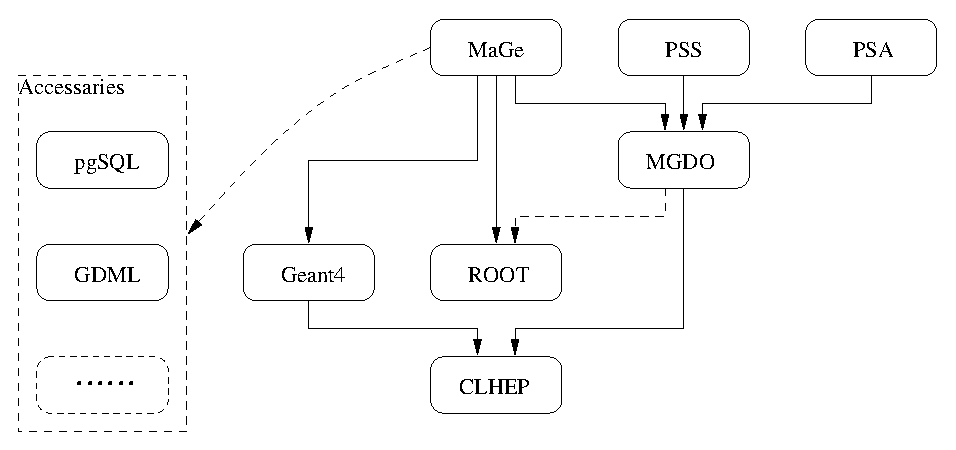
\includegraphics[width=.5\textwidth]{dependency}
  \caption{The dependencies of the software packages. Dotted lines
    indicate the optional dependencies.}
  \label{fig:dep}
\end{figure}

The dependencies determine the order of the installation, that is,
\begin{enumerate}
\item CLHEP
\item GEANT4
\item ROOT
\item MGDO
\item \mage
\end{enumerate}

\section{Getting the Packages}

\subsection{Getting CLHEP}
The \textbf{C}lass \textbf{L}ibrary for \textbf{H}igh \textbf{E}nergy \textbf{P}hysics is required for running \geant.
Go to the CLHEP web site to obtain the installation package (there are precompiled versions available):
\begin{lstlisting}
http://proj-clhep.web.cern.ch/proj-clhep/DISTRIBUTION
\end{lstlisting}
download a version newer than 1.9.x.x (2.0.4.5 is recommended by Geant4.9.3p02).

\subsection{Getting \geant}
Go to the GEANT4 web site:
\begin{lstlisting}
http://geant4.web.cern.ch/geant4/
\end{lstlisting}
download the newest version of GEANT4. If there are patches for this version,
please download them as well. GEANT4 is under development all the
time. The newer the version is, the less bugs there are.
Move the tar balls of the source codes and the patches (if there are
some) to the directory where you want to install GEANT4. Unpack the
source codes (taking version 4.8.2 as an example):
\begin{lstlisting}
  tar xfvz geant4.8.2.gtar.gz
\end{lstlisting}
Unpack the patch in the same directory:
\begin{lstlisting}
  tar xfvz patch_geant4.8.2.p01.gtar.gz
\end{lstlisting}
which will add or modify some of the GEANT4 source files.

Download the newest data files on the same web page where you download
GEANT4 source codes. Unpack them into a certain directory. Later in
the GEANT4 installation process you will be asked the place where you
put these data files.

\subsection{Getting ROOT}
To install ROOT from source you first have to get the tar file containing the source. This tar file can be found at:
\begin{lstlisting}
http://root.cern.ch/twiki/bin/view/ROOT/Download
\end{lstlisting}
The files are named root-$<$version$>$.source.tar.gz.
\begin{enumerate}
 \item Get access to the FTP area (substitute any FTP client and appropriate email address below):
\begin{lstlisting}
     ftp root.cern.ch
     User: anonymous
     Password: <your-email-address>
\end{lstlisting}
\item Go to the directory, and prepare for binary transfer of files:
\begin{lstlisting}
     ftp> cd /root
     ftp> bin
\end{lstlisting}
\item  Get the sources tar-ball (substitute the appropriate version number), and exit FTP client:
\begin{lstlisting}
     ftp> get root-<version>.source.tar.gz
     ftp> bye
\end{lstlisting}
\item Unpack the distribution:
\begin{lstlisting}
     gzip -dc root-<version>.source.tar.gz | tar -xf -
\end{lstlisting}
\end{enumerate}
\vspace{5mm}
An alternative approach is to use the cern public SVN repository to get the latest version. See
\begin{lstlisting}
http://root.cern.ch/drupal/content/subversion-howto
\end{lstlisting}
\begin{enumerate}
\item Get a specific version ($\geq$ 5.14/00), e.g.: version 5.26d:
\begin{lstlisting}
     svn co https://root.cern.ch/svn/root/tags/v5-26-00d/ root-52600d
\end{lstlisting}
\item Alternatively, checkout the head (development version) of the sources:
\begin{lstlisting}
     svn co https://root.cern.ch/svn/root/trunk root
\end{lstlisting}
\end{enumerate}
\vspace{5mm}
In both cases you should have a subdirectory called "root" in the directory you ran the above commands in.

\subsection{Introduction to SVN}
\label{sec:SVN}
SVN, known as SubVersioN control system, is a set of software used to implement a version control system which keeps track of all work and all changes in a set of files.\\
\mage is a big set of codes used to do Monte Carlo simulations for \gerda\hspace{0cm} and \majorana\hspace{0cm} experiments. \majorana\hspace{0cm} and \gerda\hspace{0cm} use SVN to manage the \mage source codes and related packages so that physicists from both sides can cooperate smoothly with each other on \mage development.\\
This chapter serves as a brief introduction on how to use SVN to help in the development of \mage.\\
Only a basic description will be given here, for more detailed information, please use the web.\\
If you know little about SVN, there is a very nice article about SVN in wikipedia:\\
\begin{lstlisting}
http://en.wikipedia.org/wiki/Apache_Subversion
\end{lstlisting}
or (in German)
\begin{lstlisting}
http://de.wikipedia.org/wiki/Apache_Subversion
\end{lstlisting}

\subsubsection{Administrators}
2004 - Xiang Liu set up the CVS server (xliu@mppmu.mpg.de).\\
2007 - 15th August. Jing Liu set up the CVS viewer and is now the CVS administrator. If you want to contact him, his e-mail is: jingliu@mppmu.mpg.de.\\
2009 - August. Jing Liu set up the SVN. The SVN administrator is Oleksandr Volynets: volynets@mppmu.mpg.de.\\

\subsubsection{Apply for an SVN account}
If you just want to browse the \mage codes, follow one of these links:
\begin{lstlisting}
http://www.mppmu.mpg.de/~gsvn/cgi-bin/viewvc.cgi
\end{lstlisting}
\begin{lstlisting}
http://www.mppmu.mpg.de/~gsvn/viewsvn/
\end{lstlisting}
You will need to know the password. Ask it from your colleagues or email to
\begin{lstlisting}
 volynets@mppmu.mpg.de
\end{lstlisting}

\vspace{5mm}
If you want to check out a copy of \mage \ and work on it, please fill out the form at
\begin{lstlisting}
 http://www.mppmu.mpg.de/~gsvn/cgi-bin/app.html
\end{lstlisting}

\subsubsection{Some Advice}
The most basic things are done. Now you can play with your copy of the codes. For a pleasant cooperation, please 
\begin{enumerate}
 \item make sure the whole package works well before committing your changes into SVN.
 \item write comments for each of your check-ins into SVN. Don't be too lazy to do so, the other users will benefit - and in the end, you will, too.
\end{enumerate}

\subsection{Getting MGDO}
MGDO package is located in the SVN repository. To get access to the SVN server, please follow the instructions in chapter \ref{sec:SVN}.

If you have already setup your SVN account for \mage, you can easily get a copy of MGDO by typing in your shell prompt:
\begin{lstlisting}
  svn co svn://pclg-soft.mppmu.mpg.de/MGDO/trunk MGDO
\end{lstlisting}
If you do this for the first time, the shell will ask you to enter your SVN password and will store this data to your
\begin{lstlisting}
  ~/.svn
\end{lstlisting}
so the next time you don't have to enter the password again.


\subsection{Getting \mage}
You can find the \mage package in the SVN repository.
To get access to the SVN server, please follow the instructions in chapter \ref{sec:SVN}.

If you have already setup your SVN account properly for \mage, you can easily get a copy of it.\\
Go to the directory in which you want to work with \mage and type there:
\begin{lstlisting}
  svn co svn://pclg-soft.mppmu.mpg.de/MaGe/trunk MaGe
\end{lstlisting}
This will check out \mage into the assigned directory which means it will copy all the codes in that directory.\\

\section{Minimum Installation}
Here is a guide aiming at helping you to compile \mage and install the
minimum software packages required by the \mage compilation.  The
guide should work for any *nix type machine (i.e. Linux, Mac OS X,
etc.) and it has been tested successfully on the following platforms:

\begin{enumerate}
\item {} Fedora Core 6 (FC 6) - x86 (Intel) and x86\_64 (AMD64) chipsets
\item {} Ubuntu 9,10 - x86 (Intel) and x86\_64 (AMD64) chipsets
\item {} Arch Linux - x86\_64 (AMD64) chipsets
\item {} Gentoo Linux - x86 (Intel) chipsets
\item {} Mac OS X (10.4) - PowerPC and x86 chipsets
\end{enumerate}



\subsection{Installation of CLHEP}
Unwind the source code tar ball in some relevant directory.
Autoconfigure and automake will aready have been run.  
Determine where the files will be installed.
Create a build directory that is NOT in the source code directory tree.
\begin{lstlisting}
cd 
/configure --prefix=
   (Note that files will be installed under /usr/local if you do not 
    specify a prefix.)
make
   (Build temporary copies of libraries and executables.)
make check
   (Run the tests.)
make install
   (Copy libraries, headers, executables, etc. to relevant 
    subdirectories under .)
\end{lstlisting}
A variety of options can be given to configure.  Below is a list 
of the options that you are likely to find most useful.
\begin{lstlisting}
  --help                  provides a partial list of options
  --prefix=PREFIX         install architecture-independent files in PREFIX
                          [default is /usr/local]
  --exec-prefix=EPREFIX   install architecture-dependent files in EPREFIX
                          [default is the same as PREFIX]
  --disable-shared        build only static libraries
  --disable-static        build only shared libraries   
  --enable-exceptions     use the CLHEP/Exceptions package
  --disable-exceptions    DO NOT use the CLHEP/Exceptions package
                          [--disable-exceptions is the default] 
\end{lstlisting}
For more information, see
\begin{lstlisting}
http://proj-clhep.web.cern.ch/proj-clhep/INSTALLATION/newCLHEP-install.html
\end{lstlisting}
A CLHEP CVS repository has also been set up:
\begin{lstlisting}
http://clhep.cvs.cern.ch/cgi-bin/clhep.cgi/
\end{lstlisting}
There is also a user's guide/reference guide:
\begin{lstlisting}
http://proj-clhep.web.cern.ch/proj-clhep/manual/UserGuide/
\end{lstlisting}

\subsection{Installation of GEANT4}
Please also read carefully the installation guide on the GEANT4 web site
before you continue:
\begin{lstlisting}
http://geant4.web.cern.ch/geant4/UserDocumentation/UsersGuides/InstallationGuide/html/index.html
\end{lstlisting}
GEANT4 needs to be informed about the environment within which it will be
installed. This can be done by setting a bunch of environment
variables manually before the compilation. GEANT4 provides a script
named \emph{Configure} to simplify this process. Once you run the
script, you will be asked some questions. GEANT4 will set up the
environment variables itself according to your answers:
\begin{lstlisting}
  cd geant4.8.2 
  ./Configure -build
\end{lstlisting}

The default answers for most of these questions work fine. However,
you need to modify some of them according to the special environment
of your computer. In order to make things clear, the whole compiling
process printed on the computer screen after you entered the above
command is shown here.
(The words between $<$ and $>$ are the
comments from the authors of this guide, which won't appear on the
screen during the real compiling process.)

\verbatiminput{g4install.log}

If everything works fine for you, you can go ahead to install GEANT4
now:
\begin{lstlisting}
  ./Configure -install
\end{lstlisting}
which will copy the compiled libraries and header files to the
installation directory you specified before.

Once libraries have been installed, the user's environment must be
correctly set up for the usage of the GEANT4 toolkit. The Configure
script provides a way to check the existing installation and provide
the correct configuration for the user's environment. Configuration
scripts env[.sh/.csh] can be generated, and should be sourced by the
final user in order to configure his/her environment according to the
performed installation. To generate the configuration scripts, the
user should run Configure placed in the installation area, as follows:
\begin{lstlisting}
  ./Configure
\end{lstlisting}
This will generate the shell script env.csh (env.sh for bash) to be
sourced or integrated into the shell login script (.tcshrc or
.bashrc). The shell script will be generated in the same directory
where you run the ``./Configure'' command. You can customize it to
specify for example the proper working directory through the variable
\$G4WORKDIR (Please refer to the later chapters for details).

\subsection{Installation of ROOT}
Don't forget to source the shell script env.csh (env.sh for bash)
generated by GEANT4 Configure script before you go on.

Please read the installation instruction on ROOT web site
carefully. An example is given below:
\begin{lstlisting}
  cd /remote/gx336-01/usr/root-5.14 (where the source codes are)
  export ROOTSYS=/remote/gx336-01/usr/root-5.14
  ./configure --disable-cern
  make
  make install
\end{lstlisting}
Before you use ROOT, please don't forget to add the following codes
into your .bashrc
\begin{lstlisting}
  export PATH=$ROOTSYS/bin:$PATH
  export LD_LIBRARY_PATH=$ROOTSYS/lib:$LD_LIBRARY_PATH
\end{lstlisting}
Or if you use tcsh, add the following to your .tcshrc
\begin{lstlisting}[language=csh]
  setenv PATH $ROOTSYS/bin:$PATH
  setenv LD_LIBRARY_PATH $ROOTSYS/lib:$LD_LIBRARY_PATH
\end{lstlisting}

\subsection{Installation of MGDO}
\subsubsection{Configuring}
MGDO is configured by going to the MGDO directory and running the configure command:
\begin{lstlisting}
  cd $MGDO
  ./configure
\end{lstlisting}
Please set your shell environment as mentioned in the previous
sections before compiling MGDO. This way, MGDO configuration system
can find all the libraries that it needs automatically. Otherwise you
have to pass these information to the configuration script by extra
configuration options. To get a list of these options, please type in
your shell prompt:
\begin{lstlisting}
  ./configure -h
\end{lstlisting}

\subsubsection{Compiling}
After a successful configuration, you can then compile MGDO by typing
in your shell prompt:
\begin{lstlisting}
  make
\end{lstlisting}
A successful compilation will create a subdirectory named ``lib''
under the MGDO directory. You will find symbol links to all the
library files under this subdirectory.

\subsubsection{Setting the Environment}
In order to let the \mage configuration system know where MGDO is
installed, you have to set a new shell environment variable named
\$MGDODIR 
\begin{lstlisting}
  export MGDODIR=/path/to/MGDO
\end{lstlisting}
in your ``.bashrc'' if you use bash, or
\begin{lstlisting}[language=csh]
  setenv MGDODIR /path/to/MGDO
\end{lstlisting}
in your ``.tcshrc'' if you use tcsh.

If you are going to use the shared libraries of MGDO, you have to add
the path of the MGDO shared libraries to \$LD\_LIBRARY\_PATH:
\begin{lstlisting}
  export LD_LIBRARY_PATH=/path/to/MGDO/lib:$LD_LIBRARY_PATH
\end{lstlisting}
if you use bash, or 
\begin{lstlisting}[language=csh]
  setenv LD_LIBRARY_PATH /path/to/MGDO/lib:$LD_LIBRARY_PATH
\end{lstlisting}
if you use tcsh.

\subsection{Installation of \mage}
\subsubsection{Configuring}
A new configure/make environment has been created to facilitate the installation process for \mage:

Go into the \mage base directory and run the command
\begin{lstlisting}
cd $MaGe
./configure [--disable-database]
\end{lstlisting}

The --disable-database flag should be passed to the configure script
if you are a GERDA user.  This flag disables support for the
PostgreSQL database used by users of \mage from the Majorana group. If the flag is
not passed to configure, and you do not have PostgreSQL on your
system, then the configure script will fail.

The configure script attempts to determine what type of system you are
using and automatically generates files important to the installation.
The script will fail if any of the required software packages are not
installed correctly and will output a message giving a suggested
course of action.  Once configure has finished successfully, \mage is
ready to be compiled.

It is important to note that if any settings have been changed
(i.e.~changes to relevant environment variables, changes in
installations of the above packages, etc.) then the configure script
needs to be rerun and the installation should be made clean (see
`Cleaning up',~\ref{sec:InstMakeClean}).


%% included by Jens Schubert, 2007/04/23
If you are a GERDA user working on one of the machines of the Max-Planck-Institute in Munich % <--- new line 
you should check whether you sourced the file \ 
{\textit{$\tilde{}$gsoft/setup.sh} } since this file sets you a valid
environment. Just type
\begin{lstlisting}
source ~gsoft/setup.sh
\end{lstlisting}
before compiling MaGe, or add it to your .bashrc file.\\
In case you are a c-shell user, type
\begin{lstlisting}
source ~gsoft/setup.csh
\end{lstlisting}
or add it to your .cshrc file.

\subsubsection{Compiling}

After a successful configure, one should run

\begin{lstlisting}
  make
\end{lstlisting}

from the \mage base directory.  

This will compile and install binaries into \$G4WORKDIR/bin/\$G4SYSTEM.

\subsubsection{Cleaning up}\label{sec:InstMakeClean}

If the installation needs to be rerun, type from the \mage base directory

\begin{lstlisting}
  make clean
\end{lstlisting}

This will remove temporary installation files and binaries for a fresh compile.

\section{Accesseries of \mage} 
% UI (GAG, JAS, etc.)
\subsection{Overview}
\mage can be enhanced by compiling against some extra packages.
\begin{itemize}
\item PostgreSQL. It is used by the \majorana \ Monte Carlo group. To
  enable it in MaGe, simply \textbf{not pass} ``--disable-database''
  option to the configuration process.
\item GDML (\textbf{G}eometry \textbf{D}escription \textbf{M}arkup
  \textbf{L}anguage). GDML is an XML-based language which describes
  the geometries of detectors in an application-independent format.
  More information about releases and getting started on GDML are available at:
\begin{lstlisting}
http://gdml.web.cern.ch/GDML/
\end{lstlisting}
\end{itemize}

\subsection{Installing PostgreSQL}
\emph{This section will undergo updates soon.} %FixME

If you are a Majorana user of \mage, then you should install PostgreSQL
(pgsql) to be able to run with all the Majorana geometries.  If you do
not wish to run a local pgsql server on your machine and only
interface with the one located at pdsf, then it is sufficient to
install the developer version of pgsql on your machine.  You can do
this by using your favorite package manager (e.g.~apt-get, fink, yum,
etc.)  and this is probably the easiest method since it will set up
your environment for you.

If you wish to run a local pgsql server, you must install the full
postgresql package (not just the developer tools).  Again, it is
simplest to install this package with your package manager.  Most, if
not all, of these distributions come with methods that will
automatically start your server of pgsql at boot time.  Please check
the documentation that comes with your distribution.
 
If you did not use a package manager, ensure that the following
environment variables are set after a successful pgsql installation:

\begin{lstlisting}[language=csh]
  setenv PGSQL_BASE_DIR /path/to/pgsql
  setenv PGSQL_LIB_DIR $PGSQL_BASE_DIR/lib
\end{lstlisting}

Setting these environment variables is unnecessary and not recommended
if the installation was performed with a package manager.

If you are running on a laptop, it is likely that you will want to
have a local version of the database installed. This way you can run
the code even when you are on a plane. To do this, do the following:
 
\begin{enumerate}

\item{} Start the server: you have to either start the server manually
  every time or setup the server to start at boot.  There should be
  methods for both in your distribution.  Please consult your
  distribution documentation.

\item{} Get the majorana database by doing (replace [username] with
  your own username) the following (you may have to sudo some of these
  commands):

 
\begin{lstlisting}
 createuser [username] (answer yes to all questions)
 createdb majorana
 pg_dump -h128.3.11.122 -p5432 -Uakbarm majorana > mjdbtemp.txt
 sed -e 's/akbarm/[username]/' mjdbtemp.txt > mjdb.txt
 psql majorana < mjdb.txt
 rm mjdb.txt mjdbtemp.txt
 \end{lstlisting}
  Test it out by doing 
\begin{lstlisting}
 psql majorana
\end{lstlisting}
and at the pgsql prompt type
\begin{lstlisting}
 psqlprompt> \dt; 
\end{lstlisting}
 This should list tables.  Quit with the command:
\begin{lstlisting}
 psqlprompt> \q; 
\end{lstlisting}


\item{}  Change MJDBProperties.txt so that 
 
\begin{lstlisting}
 databaseURL=127.0.0.1
 userName=[username]
 databaseName=majorana
 port=5432
 \end{lstlisting}
  

\end{enumerate}

\mage should now be able to access your database. Test it by running in
databaseApp (located in \$G4WORKDIR/bin/\$G4SYSTEM).
 
 
%\subsection{Performing a Standalone Installation on a Linux Machine (non-{}PDSF/Gerda)}
%\label{LinuxInstall}

% A standalone installation of \mage was successfully performed on a
%non-{}PDSF/Gerda machine at CENPA (crunch1.npl.washington.edu) running a recent
%version of Fedora Core 3 (FC3). Here is a mini-{}tutorial based on the
%experience:
 
%\begin{enumerate}

%\item{}  Make sure you have the package postgresql-{}devel installed on your
% system, and set the environment variable PGSQL\_LIB\_DIR to the
% directory containing libpq.so.



%\item{}  Install CLHEP (I used version 1.9.1.2), ROOT (v4.00.08f),
% and Geant4. 
 

%  Note about Geant4 versions: a first attempt was made at
% CENPA to use Geant4.6.2 (the currently supported version
% for \mage), but it does not compile with the version of gcc
% (3.4.2) shipped with FC3. This is a known issue, and the
% recommendation of the Geant4 team is to migrate to Geant4.7.0.
%% So Geant4.7.0 was installed. If you use an earlier version
% of gcc, you may use either.
 

%  Special Advice: when you install Geant4, I
% recommend you use the Configure script included with the
% distribution. If someone else installed Geant4 for you, track them
% down and check with them that they did this. Configure
% creates env.(c)sh scripts that you source to set all of your
% environment variables correctly. \mage depends on these environment
% variables being set correctly. So if you disregard this advice and you end
% up having trouble installing \mage as a result, you are on
% your own!
 


%\item{}  Obtain the \mage source code: follow the first few steps of 
% Chapter \ref{GettingStarted}.
% When checking out the code, it is recommend to use the option -{}P,
% as in ``cvs co -{}P \mage", to remove extraneous directories.
 


%\item{}  cd to the \mage source code root. If you want the object files,
% libraries, and binaries to be built under this directory, set the
% G4WORKDIR environment variable to the \mage source code root
% (recommended; the build may fail otherwise).
 


%\item{}  Enter the command ``make lib". The make process will complain about
% there being no release information, and will tell you that it
% thinks you are building on ``Gerda Machine X". This is just what it
% calls any non-{}PDSF computer; you may ignore this message.
 


%\item{}  A few errors were encountered due to incompatibilities with
% Geant4.7.0; these were easy to remedy by reading the 
% \href{http://geant4.cern.ch/geant4/source/ReleaseNotes4.7.0.html#7.}{Major 
% items for migration of user code}  on the Geant4.7.0 Release Notes page.  For any other errors, 
% if you don't understand them, contact the code's author.
 


%\item{}  Before making the executable, one must do ``mkdir bin" followed by
% ``mkdir bin/Linux-{}g++". This has to do with the fact that the make
% process assumes you are on a Gerda machine which already has these
% directories. 
 


%\item{}          Enter the command ``make bin". This makes the \mage executable,
% along with a utililty function databaseApp.
 


%\item{}  Contact Akbar Mokhtarani 
% (\href{mailto:amokhtarani@lbl.gov}{amokhtarani@lbl.gov})
% to allow your system to connect to the database. Send him the IP
% address(es) of the system(s) on which you are running \mage. Then
% comment-{}out all lines in the file MJDBProperties.txt, and then
% un-{}comment-{}out the last four lines to use the connection
% information for Akbar's database rather than the PDSF database.
% Once Akbar has added your system to the list of allowed IP
% addresses, test the connection by running ``bin/Linux-{}g++/databaseApp".
% If you see screens and screens of materials data fly by, and no
% error messages at the end, you are ready to run \mage.
 


%\item{}  Copy the PNNL generator files to your computer. You can find them
% on pdsf at /auto/majorana1/MJ/database/generators/PNNL. Make a
% symbolic link from \mage/dat to PNNL/dat; if you plan to run any of
% the macros in the macros directory that use the PNNL generator,
% you will need to modify the line that initializes the generator
% to point to the correct location of the PNNL directory on your
% disk.
 

%\end{enumerate}

%    Voila! Try out your exectuable by running some macros, e.g.
%   ``bin/Linux-{}g++/\mage macros/Co60.mac".
 

%\subsection{Performing a Standalone Installation on Mac OS X}

%    With some patience, \mage can run just fine on Mac OS X. The instructions
%   here used the following software versions: CLHEP 1.9.1.2, geant4.7.0,
%   and root 4.02.00. It is assumed that the user has experience
%   compiling geant4 code; if you have questions on any of these instructions
%   please \href{mailto:jasondet@u.washington.edu}{ask me}. It
%   is hoped that in the not-{}too-{}distant future, \mage will be made more
%   cross-{}platform-{}friendly and much of this will not be necessary.
 
%\begin{enumerate}

%\item{}  Install postgresql. I recommend NOT using fink for this. Instead,
% get the installation from
% \href{http://www.entropy.ch/software/macosx/postgresql}{  http://www.entropy.ch/\-software/\-macosx/\-postgresql}.
% Follow the instructions on that page. After you are done, add the following
% lines to your .(t)cshrc file (make appropriate changes for bash):
% 
%\begin{lstlisting}
%setenv PGSQL_BASE_DIR /usr/local/pgsql
%setenv PGSQL_LIB_DIR $PGSQL_BASE_DIR/lib
%\end{lstlisting}
  


%\item{}  Follow steps 2, 3, 4, 6, 7, 9, and 10 of Section~\ref{LinuxInstall}.  For step 7, replace ``Linux-{}g++" with ``\$G4SYSTEM".
 


%\item{}  Make the following changes to the GNUMakefile in the
% base-{}directory of \mage:
 
%\begin{lstlisting}
% - Near line 65: add "analysis" to PKG_SKIP.
% - Near line 130: change the line that adds libpq.so to LIBS to
%   read "LIBS = -L$(PGSQL_LIB_DIR) -lpq".
% - Near line 140: Change instances of "Linux-g++" to "$(G4SYSTEM)".
% - Near line 155: remove REL_LIB from LDFLAGS.
% - Near line 170: change the compiler option "shared" to "dynamiclib".
% - Near line 250: In the line that builds libio.so, add the root 
%   library flags to the linking flags, for example using 
%   "$(shell root-config --libs)".
%\end{lstlisting}
  


%\item{}  Make the following changes to buildTools/standard.mk
 
%\begin{lstlisting}
% - Near line 35: Add the following line after the call to the 
%   archiver in target lib:         
%   @if [ -f /usr/bin/ranlib -o -f /bin/ranlib ] ; 
%     then ranlib $(LIBDIR)/lib$(PACKAGENAME).a ;fi
%% - Near line 80: Add the option -bind_at_load to the linker flags
%   for the bin target.
%\end{lstlisting}
  


%\item{}          Near line 60 of buildTools/load\_g4.mk, the OpenGL library locations
%         are added to LDFLAGS and LOADLIBES. On my Mac, the OpenGL libraries
%         are located in /usr/X11R6/lib, so I had to change these lines to
%         read:
 
%\begin{lstlisting}
% LDFLAGS += -L/usr/X11R6/lib
% override LOADLIBES += -lXmu -lXt -lXext -lX11 -lSM -lICE
% override LOADLIBES += -lGLU -lGL
%\end{lstlisting}
  


%\item{}  In database/src/MJDatabaseUtil.cc, make the function byteswap
% return immediately. The byteswap procedure it implements is not
% necessary on Mac OS X.
 

%\end{enumerate}

%    At this point, you should be able to compile \mage by just typing ``make"
%   from the base directory. Try out your exectuable by running some macros, e.g.
%   ``bin/Darwin-{}g++/\mage macros/Co60.mac".
 

%    If you are running on a laptop like me, it is likely that you will want to have
%   a local version of the database installed. This way you can run the code
%   even when you are on a plane, and you don't have to send Akbar a new IP
%   address every time to change locations. To do this, do the following:
 
%\begin{enumerate}

%\item{}  If you followed my suggestion above and didn't use fink to install
% postgresql, then get the pgsql-{}startupitem package from
% \href{http://www.entropy.ch/software/macosx/postgresql}{  http://www.entropy.ch/\-software/\-macosx/\-postgresql}. This
% will setup the database server so that it starts up automatically
% whenever you turn on your computer and you never have to worry 
% about it. If you did use fink, you are on your own: you have to
% either start the server manually every time or write the startup
% service yourself (there are webpages on how to do this).
 


%\item{}          Get the majorana database by doing:
 
%\begin{lstlisting}
% createuser [username] (answer yes to all questions)
% createdb majorana
% pg_dump -h128.3.11.122 -p5432 -Uakbarm majorana > mjdb.txt
% psql majorana < mjdb.txt
% rm mjdb.txt
% \end{lstlisting}
%  Test it out by doing 
%\begin{lstlisting}
% psql majorana
%\end{lstlisting}
 


%\item{}  Change MJDBProperties.txt so that 
 
%\begin{lstlisting}
% databaseURL=localhost
% userName=[username]
% databaseName=majorana
% port=5432
% \end{lstlisting}
  

%\end{enumerate}

%    \mage should now be able to access your database. Test it by running
%   ../bin/Darwin-{}g++/databaseApp

\subsubsection{Installation of XERCES-C++}
GDML used to be an external package, but now it is integrated to the Geant4 toolkit. GDML depends on XERCES-C++, an XML parser written in a subset of C++. It makes it easy to give your application the ability to read and write XML data. You can find information about XERCES-C++ and the installation of it at:
\begin{lstlisting}
http://xerces.apache.org/xerces-c/
\end{lstlisting}

The easiest way to install XERCES-C++ is shown below:
\begin{lstlisting}
 tar xfvz xerces-c-3.0.1.tar.gz
 cd xerces-c-3.0.1
 ./configure --prefix=/path/to/install
 make
 make install
 export XERCESCROOT=/path/to/install
\end{lstlisting}

%%% Local Variables:
%%% TeX-master: "usersguide"
%%% End:


% -------------------------------------------------------- 
% getting started 
% --------------------------------------------------------  

\chapter{Getting Started}
\label{chapter:start}
% {\it Jing} \\
% $Id: start.tex,v 1.3 2007-10-18 11:53:27 mjelen Exp $

%%% Local Variables:
%%% TeX-master: "usersguide"
%%% End:
\label{chapter:start}


\section{The Gerda README: Getting to know Macros}
\label{sec:README}

\mage is a simulation package based on \geant. It can be run using macro files (see chapter \ref{chapter:macros}).

A lot of different macro files exist for various purposes ranging from drawing a test stand setup to simulating the background that is to be expected in the final setup of the \gerda \ experiment.

A README file was created to support new users in getting comfortable with the usage of the \gerda \ macros.

The \gerda \ README file can be found in the \gerda \ CVS repository under 
\begin{lstlisting}
/MaGe/macros/Gerda/README
\end{lstlisting}
An introduction gives a short overview on visualisation drivers used for different purposes, e.g. for presentations or for applications which require interactive features.
The macros used in the \mage \ simulations for the \gerda \ experiment are listed alphabetically and their purpose, the geometrical setup and the expected output are described in a few sentences.


 



% -------------------------------------------------------- 
% documentation  
% --------------------------------------------------------  

\chapter{Documentation} 
\label{chapter:documentation} 
{\it tba} 
\input{documentation.tex}


% -------------------------------------------------------- 
% macro commands 
% --------------------------------------------------------  

\chapter{Macro commands} 
\label{chapter:macros} 
{\it all}
%$Id: macro_commands.tex,v 1.16 2009-07-08 13:06:54 avauth Exp $
\label{chapter:MacroCommands}


The \mage \ package is a single executable program that is configured and run by
using macro files.  The usage is simple:  \mage \ is run by typing at the
command prompt 
\begin{lstlisting}
 /path/to/MaGeExecutable/MaGe /path/to/macros/SampleMacro.mac
\end{lstlisting}
\noindent where /path/to/MaGeExecutable/ is the directory of the \mage \
executable and \hbox{/path/to/macros/} is the directory of the sample macro.  Of
course this assumes you already have a macro containing your required
configurations for \mage.\\
You can also run a macro file in the \mage \ interactive mode. 
This provides the possibility to put the commands from the macro in one by one. 
This is very helpful for understanding the way the commands work and for debugging a macro script. 
Furthermore, you can implement additional commands inbetween the macro commands (e.g. if you want to change a command, but don't want to rewrite the macro).
You start the interactive mode by typing:
\begin{lstlisting}
/path/to/MaGeExecutable/MaGe 
\end{lstlisting}
Whenever \mage \ shows ``PreInit$>$'' or ``Idle$>$'', you may add new commands. There are commands which can only be given after the ``PreInit$>$''-prompt and some which require the ``Idle$>$''-prompt.\\

This chapter is all about understanding and creating
macro files so you can get \mage \ to do what you want it to do.


This chapter attempts to cover many of the macro commands one might use while
running \mage. Many are also covered in other chapters, with varying levels of
detail.  The appendix \ref{App:MacroList}
%%FIXME put in \ref and \label when appendix is written
contains a list of all messenger commands for inclusion into macro files that
have been created for use in \mage, along with explanations.  The complete list of
messenger commands native to \geant \ that one can also use is beyond the scope
of this manual.

\section{The Structure of a Macro File}
\label{sec:MacroStructure}

A macro file contains all the important messenger commands that \mage \ needs in
order to run a simulation.  Some of these parameters have ``default" values and
don't necessarily need to be set.  The bare minimum requires you to specify a
geometry, initialize the run manager, set up a primary generator of particles,
and press ``go." %%FIXME make sure this is all one needs
This would be a boring run, and you will in all likelihood want to specify much
more than this, including how the simulated data is processed and written to files.  
The structure of a macro file is divided into two parts, as follows:

\begin{itemize}
\item Set up any special manager commands \hbox{(/MG/manager/)}
\item Specify what sort of physical processes / lists you want
\hbox{(/MG/processes/)}
\item Define the geometry you want to use \hbox{(/MG/geometry/)}
\item Specify the event action commands, such as how the data are processed and
written \hbox{(/MG/eventaction/)}
\item Specify what type of primary event generator you want to use
\hbox{(/MG/generator/)}
\end{itemize}

\noindent At this point, you've told \mage \ all about the geometry setup, the
physics you're interested in, how you want the data managed and written, and
what generator to use.  Now you need to initialize the \geant \ kernel with the
messenger command 
\begin{lstlisting}
 /run/initialize
\end{lstlisting}

\noindent This tells \mage/\geant \ that it's time to build the geometry and
calculate cross sections for the physics processes you've told \mage \ to care
about.\\
You will notice that the prompt changes from ``PreInit$>$'' to ``Idle$>$'' with this initialization.\\
The structure of the macro file continues:

\begin{itemize}
\item Specify which particles you want to use, and their attributes
\item Set up any visualization scheme you want to use
\end{itemize}

\noindent Now it's time to start the run with the command

\begin{lstlisting}
 /run/beamOn n
\end{lstlisting}

\noindent where ``n" is the number of events you want to run.

This list isn't inclusive of all the types of commands you can give by macro,
but it includes all the most important ones. More information about the commands, the choice of values and the default values can be found by going into interactive MaGe mode (as indicated in the introduction of this chapter) and typing:
\begin{lstlisting}
PreInit> cd /MG/
PreInit> ls
\end{lstlisting}
You can follow the directory tree to the last leaves, the macro commands. Information about these can be obtained by:
\begin{lstlisting}
PreInit> help [macrocommand]
\end{lstlisting}
The next few sections will go into the commands in more detail.

\section{MGManager Messengers}

The manager messengers allow you to do two basic things.  You can set the
verbosity of the log you want from the output:
\begin{lstlisting}
 /MG/manager/mjlog [fatal] [error] [warning] [routine] [trace] [debugging]
\end{lstlisting}
\noindent ``Fatal" is the least verbose, while ``debugging" is the most.  It is
worth noting that these logs are specific to \mage.  You can also fiddle with
native \geant verbosity messengers like
\begin{lstlisting}
 /run/verbose j
 /event/verbose k
 /tracking/verbose l
\end{lstlisting}

\noindent where increasing integers of j, k, and l lead to increasingly detailed output
about the run, event, and tracking.  The default is 0 for silent, with maximum
output for run and event at 2 and maximum output for tracking at 5.  Be warned,
setting tracking above 2 is like drinking from a firehose, so think about how many
events you really want to run.

You can also specify what sort of random number generator seed you want.  Your
best bet is probably 
\begin{lstlisting}
 /MG/manager/seedWithDevRandom
\end{lstlisting}

\noindent which reads a seed from /dev/random.  The other options are

\begin{lstlisting}
 /MG/manager/heprandomseed [integer]
 /MG/manager/useInternalSeed [integer]
\end{lstlisting}


\section{MGProcesses Messenger} \label{macros-processes}

%%FIXME RAJ 22FEB2007: haven't looked at this yet.  Perhaps someone with more
%experience using different processes should have a look?

The MGProcesses Messenger can set the simulation ``realm" to double-{}beta decay, 
dark matter or cosmic rays.\\ 
The difference between the realms lies in the
secondary production cutoff. 
For the first two realms the distances specified in the code
are keyed to germanium, and they provide a double-{}beta production
cutoff of 100 keV and a dark matter production cutoff of 1 keV.
In the cosmic rays realm, the cuts are different in the volumes 
belonging to to the ``SensitiveRegion" and the other volumes. In particular, 
the cuts for the volumes in the sensitive region are the same than for 
the double-beta realm, while they are more relaxed everywhere else, in 
order to save CPU time (avoiding the precise tracking of particles in the
uninteresting parts of the setups). 
 

 These cutoffs specify the energy below which no secondaries will
be created (with a few exceptions, such as if the secondary
particle would annihilate, such as positrons, or if the particle
is relatively close to a volume boundary).


 The goal of establishing these different realms is to increase the
speed of the simulation when possible. Since the interesting energy
range of double-{}beta decays is much greater than that of dark
matter interactions, the simulation should not have to spend so
much time tracking secondary particles down to the lower energy

If the  ``SensitiveRegion" is not defined or 
no logical volume is registered in it, the cut-{}per-{}region 
approach has no effect in the simulation. The cuts are the same everywhere and 
correspond to about 140 keV (gammas) and 7.5 MeV (e-) in germanium. 
The code to register one logical volume in the ``Sensitive Region" is \\
\begin{lstlisting}
G4Region* sensitiveRegion =  new G4Region(``SensitiveRegion'');
sensitiveRegion-->AddRootLogicalVolume(myLogicalVolume);
\end{lstlisting}
When a volume is registered to the region, all its daughters are included too.
Don't forget to \texttt{delete sensitiveRegion;} in the destructor of the 
geometry class.\\
The MGProcesses Messenger is used as such:
 \begin{lstlisting}
 /MG/processes/realm [BBdecay] [DarkMatter] [CosmicRays]
\end{lstlisting}
The default realm is ``BBdecay".
 
Geant4 has the capability to generate and track optical photons, e.g. originated by scintillation or by 
Cerenkov emission. In the default MaGe Physics List optical photons are not generated. They can be switched 
on with the messenger command 
 
\begin{lstlisting}
 /MG/processes/optical [true] [false]
\end{lstlisting}
                    that has to be given before the 
\texttt{/\-r\-u\-n\-/\-i\-n\-i\-t\-i\-a\-l\-i\-z\-e}. In this case, 
be sure that the geometry definition contains the optical properties of materials (refraction index, absorption 
length, scintillation yield) and of surfaces (reflection index, etc.).\\
Geant4 provides two alternative sets of Electromagnetic Processes, called Standard (Std) and Low Energy (LowE). 
The LowEnergy processes include atomic effects (as fluorescence) and can track gammas, electrons and positrons 
down to 250 eV; the drawback of LowE processes is that they require a longer computing time. By default, the 
Electromagnetic processes in the MaGe Physics List are the LowE ones. One can switch to the Standard processes 
(quicker and less precise) with the messenger command 
\begin{lstlisting}
 /MG/processes/lowenergy [true] [false]
\end{lstlisting}
It must be given before the 
\texttt{/\-r\-u\-n\-/\-i\-n\-i\-t\-i\-a\-l\-i\-z\-e}.

\section{MGGeometry Messengers}\label{GeometryMessenger}
The MGGeometry Messengers are used to specify which detector is to
be simulated.  The number of geometries in use is growing, and many of them have
their own bevy of messenger commands.  This chapter won't go into all of them,
but they can be found in Appendix \ref{App:MacroList}%%FIXME make sure that I work!
The main messenger commands are:

\hbox{
\begin{lstlisting}
 /MG/geometry/detector [clover] [cloverinNaIbarrel] [solidBlock] [GerdaArray]
                       [idealCoax] [MunichTestStand] [MJ57Banger] [MPIK_LArGe] 
                       [GS_LArGe] [UWLArGe] [SLACBD] [cloverInShield] 
                       [MJRDCrystalColumn] [MJRDCryostat] [MJ17A] 
                       [MJRDBasicShield] [MCNPTest] [CERN_NA55] [WIPPn] 
                       [LLNL8x5] [GeometryFile] [Corrado]
 /MG/geometry/addMaterial
 /MG/geometry/database
 /MG/geometry/dumpG4materials
 /MG/geometry/geometryFileName
 /MG/geometry/setDetectorOffset
 /MG/geometry/setWorldHalfLen
 /MG/geometry/WorldMaterial
 /MG/geometry/EventBias/
\end{lstlisting}
} 
\vspace{5mm}

\begin{lstlisting}
 /MG/geometry/detector 
\end{lstlisting}
is used to select which geometry has to be simulated: the geometry name has to be 
chosen among the registered ones. There is \emph{not} a default geometry provided. The 
user hence \emph{must} issue the \texttt{/MG/geometry/detector} command before 
starting the run initialization. If it is not done, the \textsc{MaGe} executable 
will crash. \\

\begin{lstlisting}
 /MG/geometry/database [true] [false] 
\end{lstlisting}
allows the user to choose if the 
material table has to be read from the Majorana database (=true) (default) or from 
the local class materials/MGGerdaLocalMaterialTable (=false). \\
%

\begin{lstlisting}	
 /MG/geometry/dumpG4materials
\end{lstlisting}
can be used to print on screen all the defined materials. It works properly only
after run initialization (namely, in the ``Idle$>$'' state of
\textsc{Geant4}).  \\

\begin{lstlisting}
 /MG/geometry/geometryFileName [filename]
\end{lstlisting}
\noindent will set the file name for a file-based geometry. \\
%

\begin{lstlisting}
 /MG/geometry/setDetectorOffset
\end{lstlisting}
\noindent allows you to place the constructed detector at a specific position in
the WorldVolume.  The default is the origin. \\

\begin{lstlisting}
 /MG/geometry/setWorldHalfLen
\end{lstlisting}
\noindent allows you to set the size of the WorldVolume.  The default is a 50 m
$\times$ 50 m $\times$ 50 m cube. \\

\begin{lstlisting}
 /MG/geometry/WorldMaterial
\end{lstlisting}
determines the material used to construct the WorldVolume.  The default is air.

\begin{lstlisting}
 /MG/EventBias/
\end{lstlisting}
is a messenger directory with commands allowing the use of event biasing in
runs.  For example, one may choose to use importance sampling, as well as the
algorithm to use.
%%FIXME should point to the EventBias section that Mike Marino has been itching
%to write.


\subsection{Definition of user-specific materials} \label{subsection:materials}
The command 
\begin{lstlisting}
 /MG/geometry/addNewMaterialfilename filename
\end{lstlisting}
is used to read a material definition from an external file. It works only 
if the database is switched off. \\
The material definition should be as follows: \\
\emph{First line}: material name, density (g/cm$^3$), number of elemental components \\
The name of the material cannot contain blank spaces and must be different from 
the materials already defined in the material table. \\
The following lines (one for each component) contain: \\
 Element name, Element symbol, Z (double), A(double) and mass fraction. \\
The information written in the file is used only if the element table does not 
already contain an element with the same name. An example of a definition file 
is the following:
\begin{lstlisting}
 TelluriumOxide 5.9 2
 Oxygen O 8.0 16.000 0.201 
 Tellurium Te 52.0 127.60 0.799
\end{lstlisting}

\subsection{Debugging of geometries}
A command is available to check for overlapping volumes within the geometry.
\begin{lstlisting}
Idle> /MG/geometry/CheckOverlaps
\end{lstlisting}
The program will report on the screen the overlaps between physical volumes with their mother
volume and/or with other physical volumes at the same hierarchy level. No information is 
displayed for those volumes that are correctly placed. Additional verbosity from the 
CheckOverlaps tool, can be obtained with the command
\begin{lstlisting}
Idle> /MG/geometry/OverlapVerbosity true/false
\end{lstlisting}
(default is false).

\subsection{GDML-macros} \label{subsection:GDML-macros}

The commands used for GDML are:
\begin{lstlisting}
(reading commands, must be executed before initialization:)
/MG/geometry/GDML/sourceFile [sourcefileName]

(writing commands:)
/MG/geometry/GDML/schemaPath /path/to/gdml/schema (optional)
/MG/geometry/GDML/outputName [outputName.gdml] (optional)
/MG/geometry/GDML/outputFormat [true][false] (optional)
/MG/geometry/GDML/modularizeLevels [1][2][3]... (optional)
/MG/geometry/GDML/write (only work after initialization)
\end{lstlisting}
You can have a look at the complete set of GDML options in the interactive \mage \ mode by typing:\\
\begin{lstlisting}
MaGe
PreInit> cd /MG/geometry/GDML/
PreInit> ls
\end{lstlisting}
All the commands are displayed now. For more detailed information, type:
\begin{lstlisting}
PreInit> help [macrocommand]
\end{lstlisting}
Where [macrocommand] is any of the commands displayed.\\

\begin{lstlisting}
PreInit> /MG/geometry/GDML/sourceFile [sourcefileName] 
\end{lstlisting}
\begin{quote}
  The first command specify the position of the GDML-file.
\end{quote}
\begin{lstlisting}
Idle> /MG/geometry/GDML/schemaPath /path/to/gdml/schema
\end{lstlisting}
\begin{quote}
The second command sets your own GDML schema definition file path. /path/to/gdml/schema is the path to your schema definition. The default value is set to:
\begin{lstlisting}
http://service-spi.web.cern.ch/service-spi/app/releases/GDML/GDML_3_0_0/schema/gdml.xsd.xsd
\end{lstlisting}
\end{quote}
\begin{lstlisting}
Idle> /MG/geometry/GDML/outputName [outputName.gdml]
\end{lstlisting}
\begin{quote}
Where [outputName] is the name of the GDML output file. By default, it is the same as the detector name that you specified using the command:
\begin{lstlisting}
Idle> /MG/geometry/detector [Name]
\end{lstlisting}
\end{quote}
\begin{lstlisting}
Idle> /MG/geometry/GDML/outputFormat [true][false]
\end{lstlisting}
\begin{quote}
Set the format of the GDML output file. Candidates are ``[true][false]''.\\
true- The names of volumes, materials, etc. in the GDML output file will be concatenated with their logical address in hexadecimal format (save if you have duplicated names).\\
false - The names will correspond exactly to the ones you have in GEANT4.\\
By default, true is used.\\
\end{quote}
\begin{lstlisting}
Idle> /MG/geometry/GDML/modularizeLevels [1][2][3]...
\end{lstlisting}
\begin{quote}
Specifies the geometry levels that you want to modularize.\\
\end{quote}
\begin{lstlisting}
Idle> /MG/geometry/GDML/write
\end{lstlisting}
\begin{quote}
Dumps a Geant4 geometry to a corresponding GDML file. Be careful: this command can \textit{only} be used after the ``Idle$>$''-prompt.\\
\end{quote}
%
\subsubsection{Example Macros}
Have a look at the MaGe macro-directory to find a well commented example for GDML-macros:
\begin{lstlisting}
cd /Path/to/MaGe/macros/GDML
\end{lstlisting}
The ``GDML''  subdirectory contains the macro files ``g42gdml.mac'' and ``gdml2g4.mac''.\\
``g42gdml.mac'' is an example macro to show how to dump a \geant \ geometry into a GDML file.
You run it using the method described in the beginning of chapter \ref{chapter:MacroCommands}, in this case:
\begin{lstlisting}
$ \$ $MaGe g42gdml.mac
\end{lstlisting}
You want to test what each of the commands in a macro does? Use the interactive mode as described above.\\
``g42gdml.mac'' is well commented inside the script itself. Nevertheless, some commands and the GDML options will be explained here.\\
The macro runs with the detector ``Corrado'' (as described above).
The initialization can be accelerated by not using hadronic processes which corresponds to setting the following variable to ``true'':
\begin{lstlisting}
PreInit> /MG/processes/useNoHadPhysics true 
\end{lstlisting}
Of course, you have to run the initialization process:
\begin{lstlisting}
PreInit> /run/initialize
\end{lstlisting}
With the initialization, the prompt in MaGe changes from ``PreInit$>$'' to` ``Idle$>$''.
The tree structure of the geometry can be obtained by:
\begin{lstlisting}
Idle> /vis/open ATree
Idle> /vis/ASCIITree/verbose 1
\end{lstlisting}
This gets the names of the physical and logical volumes which are dumped and printed out by:
\begin{lstlisting}
Idle> /vis/drawTree
\end{lstlisting}
Now you have the tree structure of your geometry printed out. You may e.g. specify the levels you want to be modularized (see later).
\begin{lstlisting}
Idle> /MG/geometry/GDML/schemaPath /path/to/gdml/schema
\end{lstlisting}
This sets your own GDML schema definition file path. The default schema introduced above is also used in case of ``g42gdml.mac''.\\
\begin{lstlisting}
Idle> /MG/geometry/GDML/outputName somename.gdml
\end{lstlisting}
Where ``somename'' is the name of the GDML output file. The default name is ``Corrado.gdml''.\\
\begin{lstlisting}
Idle> /MG/geometry/GDML/outputFormat 2
\end{lstlisting}
The names of volumes, materials etc. will be the names used in \geant.\\
\begin{lstlisting}
Idle> /MG/geometry/GDML/modularizeVolumes Crystal_log Spider_log ...
\end{lstlisting}
``Crystal\_log'' and ``Spider\_log'' are the logical volumes contained in ``Corrado.gdml'' that are modularized according to ``g42gdml.mac''. They are daughter volumes of the ``Corrado''-volume.\\
\begin{lstlisting}
Idle> /MG/geometry/GDML/modularizeLevels [1][2][3][4]...
\end{lstlisting}
Specifies the geometry levels that you want to modularize. If you only use ``2'', only the second level of the tree will be used, not the first one and not the third one.\\
With:
\begin{lstlisting}
Idle> /MG/geometry/GDML/write
\end{lstlisting}
the Geant4 geometry is written to a corresponding mother GDML file, ``Corrado.gdml'' and two modularized daughter GDML files, ``Crystal\_log.gdml'' and ``Spider\_log.gdml''.\\
\vspace{5mm}
``gdml2g4.mac'' shows exemplarily how to use a GDML file in a \geant \ simulation.\\
You have to type
\begin{lstlisting}
$ \$ $MaGe
\end{lstlisting}
to go into the \mage \ interactive mode.
The command
\begin{lstlisting}
PreInit> /MG/geometry/GDML/sourceFile Crystal_log.gdml
\end{lstlisting}
specifies ``Crystal\_log.gdml'' as the GDML file that is used. You can replace this file with any GDML-file. If you want \mage \ to use the whole geometry, just insert the mother file of ``Crystal\_log.gdml'', in this case ``Corrado.gdml''.\\
Initialization is run without hadronic processes:
\begin{lstlisting}
PreInit> /MG/processes/useNoHadPhysics true 
PreInit> run initialize
\end{lstlisting}
The geometry is drawn with the visualization driver \textbf{O}pen\textbf{GL S}tored \textbf{X}:
\begin{lstlisting}
Idle> /vis/open OGLSX
Idle> /vis/viewer/set/viewpointVector 0 1 1
Idle> /vis/drawVolume
\end{lstlisting}
The generator used for simulating particles is the \textbf{G}eneral \textbf{P}article \textbf{S}ource. It is described more detailled in section \ref{sec:GPS}. In this case it shoots electrons with an energy of 100\,MeV onto the crystal.
\begin{lstlisting}
Idle> /MG/generator/select SPS
Idle> /gps/particle e-
Idle> /gps/energy 100 MeV
Idle> /gps/position 1 1 1
Idle> /gps/direction 0 1 1
\end{lstlisting}

\begin{lstlisting}
Idle> /vis/scene/add/trajectories
Idle> /run/beamOn 10
\end{lstlisting}
Now you should see a detector setup with particle trajectories.\\
\vspace{5mm}\\
``g42gdml.mac'' gives out three GDML-files: ``Corrado.gdml'', ``Crystal\_log.gdml'' and ``Spider\_log.gdml''. These can be displayed running the ROOT-macro ``drawGDML.C'':
\begin{lstlisting}
$ \$ $ROOT
ROOT[].x drawGDML.C(``filename.gdml'')
\end{lstlisting}
``filename.gdml'' is any of the three files produced by ``g42gdml.mac''.\\

\section{MGOutput Messengers}
In order to retrieve the relevant information from the simulation, the user should also 
specify which output scheme has to be used. Output classes can give either a ROOT file 
or an ASCII file.\\
The commands to define the output schema and to retrieve the name are:
\begin{lstlisting}
 /MG/eventaction/rootschema name
 /MG/eventaction/getrootschema
\end{lstlisting}
A number of alternative output schemes are presently available in \textsc{MaGe}: LANLCloverNoPS, 
LANLCloverSteps, LANLCloverInNaIBarrel, solidBlock, GerdaArray,
GerdaArrayWithTrajectory, LArGeNoPS, G4Steps, MCEvent, 
GerdaTestStand, GerdaTestStandSimple, GerdaArrayOptical, GerdaArrayCalibration, 
MPIK\_LArGe, GerdaTeststandCoincidence, SLACBD, Shielding, GSS, MCNPTest, 
CERN\_NA55, GerdaTeststandSiegfried, GerdaTeststandSiegfriedCoincidence, 
NeutronYield and DetectorEfficiency. \\
This must be done with care, as the output class can be tied to the detector choice, and 
there is so far no internal checking to make sure the output class and detector choice.\\
The name of the output file is also set via messenger, using the command
\begin{lstlisting}
 /MG/eventaction/rootfilename filename
\end{lstlisting}
The same command works for ROOT and ASCII output file. \\
\textsc{MaGe} correctly runs (e.g. for testing purposes) even if the output class is 
not specified.

\begin{lstlisting}
 /MG/eventaction/reportingfrequency
\end{lstlisting}
determines how often the output tells you which event it is processing.

\begin{lstlisting}
 /MG/eventaction/writeOutFileDuringRun
 /MG/eventaction/writeOutFrequency
\end{lstlisting}
allow for writing to the file during the run.  The default frequency that it
writes is the same as the reporting frequency.


\section{MGGenerator Messengers}

A simulation is only useful if you actually fire particles at things.  Using the
generator macros is how you set this up.  The only generator messenger you need
to issue before \texttt{/run/initialize} is
\begin{lstlisting}
 /MG/generator/select [PNNLiso] [RDMiso] [TUNLFEL] [G4gun] [decay0] [cosmicrays] 
                      [musun] [SPS] [neutronsGS] [wangneutrons] [AmBe] 
                      [MuonsFromFile] [sources4a] [GSS]
\end{lstlisting}
which selects the generator engine you will use.  There is much more information
about these generators in Chapter \ref{chapter:generators}

The other basic messenger commands:
\begin{lstlisting}
 /MG/generator/name
\end{lstlisting}
returns the name of the generator.

\begin{lstlisting}
 /MG/generator/position
\end{lstlisting}
This command will set the initial particle position (for point distributions
only) for all the generators.


\begin{lstlisting}
 /MG/generator/confine [noconfined] [volume] [volumelist]
 /MG/generator/volume [noconfined] [volume] [volumelist]
 /MG/generator/volumelist
 /MG/generator/volumelistfrom
 /MG/generator/volumelistto
\end{lstlisting}
allow you to confine primary vertices to within physical volumes in your
geometry.   For example, a generator that samples a 

\begin{lstlisting}
 /MG/generator/gsspositionsfile
 /MG/generator/gsseventnumber
 /MG/generator/gssoffset
\end{lstlisting}



volume
position





\section{Cone Cut for secondary gammes} \label{section:GammaConeCut}

Tracks of any gammas (primary and secondary) can be killed if the momentum vector of the photon does not point 
towards some position within a certain angle. \\
This can be used to run the simulation more efficient if the volume 
in which the gammas are generated is far away from crystal array. \\

Example:

\begin{lstlisting}
 /MG/output/killGammasOutsideCone true
 /MG/output/GammaConeCut_ArrayCenter 0 0 19.5 cm
 /MG/output/GammaConeCut_StartCutRadius 80 cm
 /MG/output/GammaConeCut_MaxAllowedOpeningAngle 45 deg
\end{lstlisting}

When the Gamma-Cone-Cut feature is enabled, all gammas not pointing to the position \textit{GammaConeCut\_ArrayCenter} within the angle 
given by \textit{GammaConeCut\_MaxAllowedOpeningAngle} will be killed, if the primary vertex of the photon 
is outside a spherical range \textit{GammaConeCut\_StartCutRadius} of this position.



%%% Local Variables:
%%% TeX-master: "usersguide"
%%% End:



% -------------------------------------------------------- 
% generators 
% --------------------------------------------------------  

\chapter{Generators} 
\label{chapter:generators} 
{\it Luciano} 

\section{Choosing a generator}

Presently eleven alternative generators have been implemented in \textsc{MaGe}.
The actual generator to be used has to be set via the macro command

\begin{lstlisting}
 /MG/generator/select [PNNLiso] [RDMiso] [TUNLFEL] [G4gun] [decay0]
   [cosmicrays] [musun] [SPS] [neutronsGS] [wangneutrons] [sources4a]
   [AmBe] [MuonsFromFile] [GSS]
\end{lstlisting}

\textsc{G4Gun} is the default G4ParticleGun provided by Geant4.

\begin{table}[tp]
\caption{Summary table of the generators available in \mage}
\label{Table:generators}
\begin{center}
\begin{tabular}{|c c|}
\hline
Events to be generated & Generator \\
\hline
Double beta decay ($2\nu$ or $0\nu$) & decay0 \\
\hline
Radioactive contaminations & G4gun \\
 & PNNLiso \\
 & RDMiso \\
 & decay0 \\
 & SPS \\
\hline
Cosmic-ray muons & cosmicrays \\
 & musun \\
 & MuonsFromFile \\
\hline
Cosmogenic neutrons & neutronsGS (for LNGS) \\
 & wangneutrons \\
\hline
Neutrons from fission and ($\alpha$,n) & neutronsGS (for LNGS) \\ 
 & Sources4a \\
\hline
Neutrons (and $\gamma$-rays) from AmBe & AmBe \\
\hline
TUNFEL beam & TUNFEL \\
Surface Contamination & GSS \\
\hline
\end{tabular}
\end{center}
\end{table} 

\section{AmBe Generator}
%FixME owned by Alexis
The americium beryllium (AmBe) generator is a point source of neutrons and 
gammas. The AmBe neutron spectrum used comes from Figure 5 of Marsh,
Thomas, and Burke, "High resolution measurements of neturon
energy spectra from Am-Be and Am-B neutron sources", Nucl. Inst.
and Meth. A 366 (1995) 340-348. Gamma energies are taken from the $^{12}$C 
level structure, at
from http://www.nndc.bnl.gov/nudat2/getdataset.jsp?nucleus=12C.
Choice of gammas depending on neutron energy is taken from Figure 3 of 
Geiger et al., Nucl. Inst. and Meth. 131 (1975) 315.
 
  


\section{PNNL Radioactive Decay Chain Generator}

\subsection{General description}

 The PNNL radioactive decay chain generator consists of a set of G4 classes for
sampling charged particles (beta or alpha) and associated gammas arising from 
the decay of any radioisotopes in a user-{}specified radioactive decay chain.
Information returned by the generator is currently limited to the charged
particle type (beta+/-{} or alpha), charged particle energy, number of ``cascade"
gammas, and a list of gamma energies.  Currently the code is limited to linear
decay chains, i.e. multiple branch points in a decay chain yielding distinct
nuclear species are not (easily or naturally) supported.  (If only gammas are
of interest, however, a multiple-{}branch kludge is possible if the branches
merge in a common daughter.)  The generator code requires as input the gamma 
cascade branching fractions for each radioisotope in the decay chain (one
ascii-{}format file per radioisotope), and a master ``decay chain" ascii-{}format
file specifying the number of radioisotopes in the chain, the decay half-{}lives
for each isotope and the names of each isotope's cascade file.  The cascade
branching fractions can be calculated using the tool CrazyInput, written by 
J.E. Ellis and A. Valsan of PNNL.  As currently implemented, setup of the 
generator requires running CrazyInput once for each radioisotope in the decay 
chain of interest.  The ascii-{}format files output by CrazyInput are then
collected in a single directory and read by the generator upon initialization.
Terminology used in this paragraph is explained in more detail below.
 

 The main object/data structure in the generator is a DecayChain object, 
representing e.g. the Thorium decay chain (consisting of the radionuclides 
Th-{}232, Ra-{}228, Ac-{}228, ..., Pb-{}208). The DecayChain's primary 
responsibilities are to serve as a container for radioisotopes, embodied in 
Radioisotope objects, to calculate the relative decay probability for each 
member isotope of the chain based upon the grow-{}in age of the source, and to 
sample appropriately from each Radioisotope object's decay.  Each Radioisotope
object can decay by either beta(+/-{}) or alpha emission, accompanied by the 
emission of one or more ``cascade" gammas from the daughter nucleus.  A cascade
is defined as a single decay scheme of a single radioisotope: For example, 
beta decay to a given excited state in the daughter nucleus, followed by 
emission of N gammas of energy E1, E2, ..., EN.  (Currently no time 
information is associated with the cascade gammas, which are assumed emitted 
in coincidence.) In general, a single radioisotope can decay via multiple 
cascade schemes.  Within the generator framework, each Radioisotope object 
thus contains one or more Cascade objects, each of which contains all of the 
information necessary for setting up and sampling from e.g. a beta decay 
energy distribution specific to that cascade decay scheme.  Each Cascade 
object also contains a list of coincident gammas associated with the cascade.
Each Radioisotope object stores a list of branching fractions for the set
of cascade it contains, and its primary responsibility is to sample from
the set of cascades associated with it when interrogated by the DecayChain
object for the current event.  In turn, a particular Cascade object ``knows"
how to sample from the beta distribution associated with it.  (Mono-{}energetic
alphas can also be associated with a cascade scheme.)  The logical structure 
of the generator is thus a nesting of data structures: a DecayChain object 
contains one or more Radioisotope objects, which in turn contain one or more 
Cascade objects.  These objects are described in the classes 
MGGeneratorPNNLDecayChain, MGGeneratorPNNLRadioisotope, and 
MGGeneratorPNNLCascade, respectively.
 

 The three main tasks of the PNNL generator are as follows: (1) Upon 
initialization, read a set of user-{}supplied files defining the decay chain and
specifying the set of cascade schemes appropriate to each radioisotope in the 
chain.  (2) Determine the relative activities (via standard Bateman equation 
calculations) of each radioisotope in the decay chain, given a user-{}supplied
list of the half-{}lives of each isotope in the chain and the grow-{}in time, T,
appropriate for the material.  It is assumed that T=0 corresponds to a material
consisting entirely of the isotope at the head of the chain.  (3) For event
sampling, select the next radioisotope to decay (based upon relative activities
of each isotope in the chain), and for that isotope, select a given cascade
decay scheme (based on cascade branching fractions determined by the CrazyInput
tool).  The energy of the decay beta (or the single energy of an alpha) is 
then sampled from an appropriate distribution and the list of corresponding
decay gammas (if any) retrieved from the appropriate Cascade object.  The 
generator returns a CascadeEvent object to the calling routine (e.g. the 
GeneratePrimaries member function of the PrimaryGeneratorAction class) for
the current event, and all information (e.g. particle types and energies) 
relevant to the radioactive decay can be extracted from this simple data 
structure in preparation for adding particles to the tracking stack.
 

\subsection{Using the generator}

\subsubsection{Setup}

 Setting up the generator currently requires (1) creating a set of ascii-{}format 
files (one for each radioisotope in the decay chain of interest) using the 
CrazyInput cascade branching-{}fraction calculation tool; (2) collecting these 
files in a convenient sub-{}directory; and (3) creating a master ``decay chain 
file" to describe to the generator the number of isotopes in the chain, the
half-{}life of each isotope, and the files listing the cascade branching
fractions for each isotope.
 

 An example cascade branching-{}fraction file for Tl-{}208 is displayed below.
 

\begin{lstlisting}
 208.0   81.0   10
 0.49499E+00    1.79626   1   1   2
  0.58319  2.61453
 0.23966E+00    1.28556   1   1   3
  0.51077  0.58319  2.61453
 0.12545E+00    1.51889   1   1   2
  0.86056  2.61453
 0.96121E-01    1.51889   1   1   3
  0.27736  0.58319  2.61453
 0.18924E-01    1.03304   1   1   3
  0.76313  0.58319  2.61453
 0.11496E-01    1.03304   1   1   4
  0.25261  0.51077  0.58319  2.61453
 0.39991E-02    1.07420   1   1   4
  0.21140  0.51077  0.58319  2.61453
 0.37982E-02    1.28556   1   1   2
  1.09390  2.61453
 0.31466E-02    1.28556   1   1   3
  0.23336  0.86056  2.61453
 0.24109E-02    1.28556   1   1   0
\end{lstlisting}

 The first line of the file lists A, Z, and the number of cascades contained
in the file.  Each cascade consists of two lines of input.  The first
line lists, in order, the branching fraction for the cascade, the endpoint
energy for the beta decay spectrum (or the alpha-{}particle energy) in MeV, the 
charged particle type (0 for alpha, 1 for beta, 2 for positron), the angular
momentum change, ``delta(L)" (in units of hbar), suffered by the nucleus in 
the decay, and the number of gammas associated with the de-{}excitation cascade 
emitted by the daughter nucleus.  The second line of the cascade description
lists the energies of the cascade gammas (MeV).  In the example file, 10 
cascade decay-{}schemes for Tl-{}208 are listed.  Reading from the second and 
third lines of the file, the first decay scheme is beta decay with an endpoint
energy of 1.79626 MeV and delta(L) of 1.  The beta is accompanied by 2 cascade
gammas of energy 0.58319 and 2.61453 MeV, respectively.
 

 In general, for a decay chain consisting of N radioisotopes, each radioisotope
must be described by a cascade branching fraction file in the format shown
above.  In addition to these files, an ascii-{}format ``decay chain file" must
be supplied to inform the generator of the general decay chain structure.  An
example file for the Th-{}232 decay chain is exhibited below.
 

\begin{lstlisting}
10
 1  Th-232   1.41e10  y  dat/cascades_232Th.dat
 2  Ra-228   5.75     y  dat/cascades_228Ra.dat
 3  Ac-228   6.15     h  dat/cascades_228Ac.dat
 4  Th-228   1.910    y  dat/cascades_228Th.dat
 5  Ra-224   3.64     d  dat/cascades_224Ra.dat
 6  Rn-220  55.0      s  dat/cascades_220Rn.dat
 7  Po-216   0.15     s  dat/cascades_216Po.dat
 8  Pb-212  10.64     h  dat/cascades_212Pb.dat
 9  Bi-212  60.6      m  dat/cascades_212Bi.dat
10  Tl-208   3.05     m  dat/cascades_208Tl.dat
\end{lstlisting}

 The first line in the decay chain file lists the number of radioisotopes in the
chain (10 in this example).  Each radioisotope is described in a single line.
The first entry in a radioisotope line is an (arbitrary) integer index which 
is not used by the code but may be useful to the user.  The second entry is
a string isotope label, used only in diagnostic messages output by the 
generator.  The third and fourth entries specify the decay half-{}life and the
units of the entry: (y,d,h,m,s) for (year, day, hour, minute, and second)
respectively.  The final entry lists the name and path of the cascade branching
fraction file for the radioisotope, relative to the directory in which the
G4 code is to be run.  (This ``main" directory will contain e.g. a macro file
containing G4 messenger commands, as well as the master decay chain file.)
 

 In summary, note that the user must (currently) construct the master decay 
chain file by hand.  The cascade branching-{}fraction files, one for each 
radioisotope, are generated by running the CrazyInput tool.  Once these files
are available and the decay chain file has been constructed, generator setup 
for the particular decay chain of interest is complete.
 

\subsubsection{Initializing the generator}

 Once the required set of input files has been prepared, initialization of the 
generator is controlled by two messenger commands in a G4 macro file, as
demonstrated in the example which follows:
 

\begin{lstlisting}
 /generator/PNNL/init Th232_DecayChain.dat
 /generator/PNNL/setSourceAge 5.0
\end{lstlisting}

 In this example, the command ``/generator/PNNL/init Th232\_DecayChain.dat"
informs the primary event generator code that the PNNL radioactive decay
chain generator will be used in the G4 run, and initializes the generator with
the name of the decay chain control file.  Typically this control file will
reside in the same directory as the G4 macro file controlling the batch run.
The command ``/generator/PNNL/setSourceAge 5.0" sets the source grow-{}in age
to 5.0 years in this example.  Recall that the relative activities of each
radioisotope in the decay chain are calculated using the Bateman equations,
with the assumption that time T=0 corresponds to a source consisting solely
of the material at the head of the decay chain (Th-{}232 in this example.)  If
the setSourceAge messenger command is not issued, the default value for the
grow-in age is 0.  In this case, only radioactive decays from the isotope at 
the head of the chain are sampled by the generator.
 

 In summary, the general messenger command structure is as follows:
 

\begin{lstlisting}
 /generator/PNNL/init [master decay chain filename]
 /generator/PNNL/setSourceAge [source grow-in age in years]
\end{lstlisting}

\section{Decay0 Generator}

\textsc{Decay0} is a primary generator developed by Vladimir I. Tretyak. 
It can generate two-neutrinos double beta decay events, and neutrinoless double beta decay 
according to a large number of theoretical models and background events from the most common 
$\gamma$/$\beta$ sources (low-probability transitions are included); it can also produce 
generic $\beta$ spectra and mono-energetic particles. The most recent version of 
\textsc{Decay0} accounts for the angular correlation between $\gamma$-rays emitted in 
$^{60}$Co and in the two-neutrino double beta decay of $^{76}$Ge to the $0^{+}_{1}$ 
excited state of $^{76}$Se (1122~keV).\\ 
\textsc{Decay0} accounts for the kinematic of the final state (i.e. momenta of all 
the particles) and for the time, which is relevant for chains or delayed 
de-excitation (e.g. $^{137}$Cs+$^{137m}$Ba). It is a \texttt{Fortran} standalone 
program and the MG generator class (MGDecay0Interface.hh) reads from the ASCII files 
dumped by it: the user must take care that the file contains enough 
events for the Geant4 simulation (otherwise the program will give an 
exception). \\
\textsc{decay0} is not a part of \mage, but the \texttt{Fortran} source code for 
the most recent version is included in the CVS repository, in the directory \texttt{GETools}. 
It must be compiled and linked with the CERN Fortran libraries. \\
%
The \textsc{Decay0} generator is instantiated with the macro command:
%
\begin{lstlisting}
 /MG/generator/select decay0
\end{lstlisting}
%
and the file to be read is set with the command  
%
\begin{lstlisting}
 /MG/generator/decay0/filename myfile.txt
\end{lstlisting}
%
The file name must be set before the \texttt{/run/beamOn}.
%
\section{Cosmic rays generator}\label{Chapter:cosmic_rays}
%FixME owned by Luciano
It is used to generate high-energy muons with the characteristic spectrum 
of cosmic rays in underground sites. 
The primary position is sampled from a disk of radius $r$ (default = 8 m) placed 
at the height $h$ (default = 8.1 m). Both these values can be changed via messenger.\\ 
The energy spectrum is sampled using the analytical parametrization of  
Lipari and Stanev~\cite{Lipari:1997}, which applies to rock depths 
between 1 km w.e. and 10 km w.e. The spectral index of the muon spectrum can be 
3.7 (standard), 2.7 (Prompt sources, e.g. charm decay) or 2.0 (Exotic sources). The 
defaults are 3400 m w.e. (Gran Sasso depth) and 3.7 respectively. \\
The angular spectrum is sampled according to the measurements performed at Gran Sasso 
by the MACRO experiment. The MACRO data are loaded from an ASCII file in the 
directory \texttt{\$MGGENERATORDATA}. If the file is not present, the distribution is 
sampled according to $\cos^{-1}\theta$, as described in Ref.~\cite{Lipari:1997}. 
In the latter case, a warning message is printed on the screen.

The cosmic ray generator is instantiated with the macro command:

\begin{lstlisting}
 /MG/generator/select cosmicrays
\end{lstlisting}

The commands to change the parameters of the generator are:
\begin{lstlisting}
 /MG/generator/cosmicray/radius radius [unit]
 /MG/generator/cosmicray/height radius [unit]
 /MG/generator/cosmicray/depth  depth [unit]
 /MG/generator/cosmicray/index index
\end{lstlisting}

for radius, height, depth (with unit) and spectral index respectively.
 
\section{The muons from file generator}\label{Chapter:muons_from_file}

This generator was developed, to allow the user to select muons from a file, instead 
of using the cosmic rays generator, that was introduced in the previous chapter \ref{Chapter:cosmic_rays}.
It reads the starting position, the direction and the energy of the muon from a file with a structure like:
\begin{lstlisting}
 pos(x) pos(y) pos(z)  dir(x) dir(y) dir(z)  energy
\end{lstlisting}
with the three dimensions of the starting position \textit{pos(x,y,z)}, the three elements of the direction
vector \textit{dir(x,y,z)} and the \textit{energy} of the muon. It was mainly used to simulate a set of muons, 
that were identified as dangerous, i.e. during their simulation, an energy deposition around 2 MeV in the germanium crystals
was registered. An example of a small file is given in tabular \ref{Tab:muon_example}.
\begin{table}[tp]
\caption{Example table of some dangerous muons for \mage. The header must not be included into the file.}
\label{Table:generators}
\begin{center}
\begin{tabular}{|c|c|c|c|c|c|c|}
\hline
 pos(x) & pos(y) &  pos(z) & dir(x) & dir(y) & dir(z) & energy \\ \hline \hline
1199.75 & 69.6281 & 810 & -0.836506 & -0.0649792 & -0.544091 & 370888 \\
200.717 & 541.989 & 810 & -0.301985 & -0.469251 & -0.829825 & 914548 \\
305.095 & -292.536 & 810 & -0.355895 & 0.34182 & -0.869769 & 1.31997e+06 \\
-1476 & -727.268 & 810 & 0.812514 & 0.390033 & -0.433238 & 570688 \\
-474.305 & -731.501 & 810 & 0.421681 & 0.602593 & -0.677545 & 213939 \\ \hline
\end{tabular}
\end{center}
\end{table}

The muons from file generator is initiated with the macro command:

\begin{lstlisting}
 /MG/generator/select MuonsFromFile
\end{lstlisting}

The commands to change the parameters of the generator are:
\begin{lstlisting}
/MG/generator/MuonsFromFile/filename file
\end{lstlisting}

to change the name of the file, from which the muons are read in. The files have to be stored 
into the MGGENERATORDATA folder. 




\section{MUSUN Generator}
\textsc{MUSUN} is a primary generator developed by Vitaly Kudryavtsev and described 
in \cite{Kudryavtsev:1997}. It is \texttt{Fortran}-based and it is able to track 
high-energy muons through large thicknesses of rock, to obtain the muon spectrum (energy and 
direction) inside an underground Laboratory. It can also take into account 
the depth profile of the specific Laboratory, if available, in order to 
reproduce the possible asymmetries in the azimuth distribution. The \mage  
generator is istantiated with the command:
\begin{lstlisting}
 /MG/generator/select musun
\end{lstlisting}
%
It reads the event kinematic parameters (energy and direction) of 
the primary muon from an ASCII file, whose name (and path, if it is not 
in the current directory) has to be provided using the macro command 
%
\begin{lstlisting}
 /MG/generator/musun/filename myfile.txt
\end{lstlisting}
%
The primary position is sampled from a disk of radius $r$ (default = 8 m) placed 
at the height $h$ (default = 8.1 m). Both these values can be changed via messenger, 
using the same commands described in the previous section for the CosmicRay 
generator, i.e. 
%
\begin{lstlisting}
 /MG/generator/cosmicray/radius radius [unit]
 /MG/generator/cosmicray/height height [unit]
\end{lstlisting}
  
\section{NeutronsGS generator}
This generator produces neutrons induced by natural radioactivity and interactions of cosmic-ray 
muons in the rock. Energy is sampled according to the spectrum at Gran Sasso reported 
in Ref.~\cite{Wulandari:2004}. The generator is instantiated with the command 
 
\begin{lstlisting}
 /MG/generator/select neutronsGS
\end{lstlisting}

The data are read from ASCII files, that are looked for in the directory 
\texttt{\$MGGENERATORDATA}. 
It is possible to generate either the low-energy component from 
fission and ($\alpha$,n) from the rock or the high-energy component induced 
by muon interactions in the rock. The latter is the default. The spectrum to 
be generated can be selected via messenger:
\begin{lstlisting}
 /MG/generator/neutrons/fission [true] [false]
\end{lstlisting}
If the value \texttt{true} is assigned, the low-energy component produced by natural 
radioactivity in the rock is considered.
The fission/($\alpha$,n) neutrons are considered to be isotropic, while the 
angular distribution of the high-energy component is sampled according to 
\cite{Wulandari:2004}. 
The position of the primary tracks is sampled from the 
upper surface, the lower surface or the lateral surface of a cylinder; it 
can be set with the command:
\begin{lstlisting}
 /MG/generator/neutrons/direction [roof] [floor] [walls]
\end{lstlisting}
The dimensions of the cylinder are 8.0~m radius and 8.0~m height. The defaults 
can be changed with the commands
\begin{lstlisting}
 /MG/generator/neutrons/radius radius [unit]
 /MG/generator/neutrons/height height [unit]
\end{lstlisting}
%

\section{Sources-4A Generator}
\textsc{Sources-4A} is a \texttt{Fortran}-based generator of neutrons produced 
in a given material by fission and by ($\alpha$,n) reactions on light elements. 
It has been developed by the LANL; a large number of cross section tables for 
various elements has been recently added in the context of the ILIAS 
EU work. The code calculates the energy spectrum of the emitted neutrons; 
the angular distribution is assumed to be isotropic. The explicit 
tracking of the neutron (out of its source, for instance) is not done 
by \textsc{Sources-4A} but has to be performed using \mage\ and \geant.\\ 
The output from \textsc{Sources-4A} is the absolute energy distribution of neutrons; 
the total production rate is expressed in \mbox{neutrons cm$^{-3}$ s$^{-1}$}. The name of the 
output file from \textsc{Sources-4A} containing the absolute energy spectrum is \texttt{tape7}. 
The \mage \ generator is istantiated with the command
 
\begin{lstlisting}
 /MG/generator/select sources4a
\end{lstlisting}
In the default case, the data file to be read is called \texttt{tape7} and it is 
looked for in the current directory. The file name can be alternatively specified 
(with its path) using the command 
\begin{lstlisting}
 /MG/generator/sources4a/filename myfile.txt
\end{lstlisting}
The generator also works if the normalized energy spectrum (called 
\texttt{tape8} in the default case) is used.\\ 
The only limitation of the generator is that the lower egde of the lowest-energy 
bin must be zero. The generator does not take care of the position sampling of the 
neutron; in most case, it will be appropriate to use the uniform position sampling in 
a given volume, which is described in Sect.~\ref{Section:positionsampling}. 

\section{General Particle Source}\label{sec:GPS}
{\em Note:  The GPS has many, many options, not all of which are covered in this
manual.  For a complete list, look at the \geant \ source code.  Once you give
that up, look at the much more accessible GPS user's manual at
\hbox{http://reat.space.qinetiq.com/gps/}.  It explains everything and also contains many example
macros.} 

The \geant \ General Particle Source (GPS) was designed to supplant the G4Gun as a
general source for any particles you might want to use.  It also allows for
position sampling, angular and energy distributions, and multiple sources.  To use the GPS, the messenger command is
%
\begin{lstlisting}
 /MG/generator/select SPS
\end{lstlisting}
The GPS can sample from several types of planes(circle, annulus, ellipsoid,
square, rectangle) and surfaces/volumes(sphere, ellipsoid, cylinder,
parallepiped).   Messenger commands set the sizes, positions, and attributes of
the original positions.  Some examples are
%
\begin{lstlisting}
 /gps/position 1.0 2.0 2.5 cm
 /gps/pos/type Plane
 /gps/pos/shape annulus
 /gps/pos/radius 5.0 cm
 /gps/pos/inner_radius 3.0 cm
\end{lstlisting}
%
The angular and energy distributions can also be customized.  The choices for
angular distributions are isotropic,
cosine-law, or user-defined.  You can also choose parallel beam or a diverging
accelerator beam.  For energy distributions, you can choose from mono-energetic,
linear, exponential, power-law, gaussian, bremsstrahlung, black body, and cosmic
diffuse gamma ray.  Some example messenger commands utilizing these(taken from
Example 13 in the GPS user's manual,
\hbox{http://reat.space.qinetiq.com/gps/examples/examples.htm}):
%
\begin{lstlisting}
 /gps/ang/type cos
 /gps/ene/type Exp
 /gps/ene/min 2. MeV
 /gps/ene/max 10. MeV
 /gps/ene/ezero 6.
\end{lstlisting}
%
The GPS uses the \geant \ native radioacative decay module (RDM).  To set up an
ion and set limits on it's decay, 
\begin{lstlisting}
 /gps/ion <Atomic Number> <Mass Number> <Ionic Charge> <Excitation Energy>
 /grdm/nucleusLimits <Amin> <Amax> <Zmin> <Zmax>
\end{lstlisting}

To set up
a radioactive ion, say $^{238}$U, and let it decay to $^{222}$Rn, the messenger
commands would be
%
\begin{lstlisting}
 /gps/particle ion
 /gps/ion 92 238 0 0
 /gps/energy 1e-20 eV
 /grdm/nucleusLimits 222 238 86 92 
\end{lstlisting}
%
\noindent

\section{Position sampling} \label{Section:positionsampling}
Only a few of the generators described above take care of sampling the initial position of 
the primary particle. Notably, they are: TUNFEL, MUSUN, CosmicRays, NeutronsGS,
and \hbox{SPS}/\hbox{GPS}(General Particle Source).
%%FIXME is this accurate?  RAJ 21Feb2007
For 
all the others, the source is considered to be a fixed point.
The default is the origin of the coordinate system, but it can be set (for any generator) 
with the macro command
\begin{lstlisting} 
 /MG/generator/position coordinates [unit]
\end{lstlisting}
The command has no effect on the TUNFEL, MUSUN, CosmicRays and NeutronsGS generators, that 
internally overwrite the position of the primary particle. For the G4gun generator only, the 
command 
\begin{lstlisting} 
 /gun/position coordinates [unit]
\end{lstlisting}
can also be used.  The General Particle Source (GPS) has all of the features of
the G4gun, but also much more in the way of position sampling and angular/energy
biasing.\\
%
\subsection{Uniform sampling} 
For some applications (e.g. simulation of internal contamination) it 
is useful to sample the position of the primary event uniformly within a given 
physical volume or a given skin surface. 
The \mage \ package includes an algorithm for this purpose. 
The confinement level (noconfined, volume, surface) is set with the command: 
 
\begin{lstlisting}
 /MG/generator/confine   [noconfined] [volume] [surface] [volumelist]
\end{lstlisting}

The default is \texttt{noconfined} (e.g. primary generated in a fixed position). 
If the confinement level is set to \texttt{volume}, the physical volume 
has to be set with the command 
 
\begin{lstlisting}
 /MG/generator/volume volumename
\end{lstlisting}

\noindent where \texttt{volumename} is the name of an existing physical volume. This command has 
to be called after /run/initialize. If the volume name is not unique (e.g. replicas exist), 
the copy numbered ``0" will be taken into account.  The surface confinement
level has not been implemented in this context, but an alternate method exists
and is covered in Section \ref{sec:surfacesampling}. \\

\subsubsection{Confinement in geometrical volumes or surfaces}
It is also possible to sample the position of the primary event uniformly in a geometrical 
volume (e.g. a spherical shell, or a cylinder) or a geometrical surface (e.g. a disk, or a sphere). 
Although this functionality is already provided by the General Particle Source generator 
(see sect.~\ref{sec:GPS}), the General Particle Source treats also direction sampling and it is 
not possible to use the tools described in Sect.~\ref{sec:direction}, as the sampling of the 
direction of the primary particle within a given angle from a target position. The position sampling 
over a geometrical volume/surface, as provided by \mage, can be coupled with the tools for 
direction sampling.

The confinement level is set with the command 
\begin{lstlisting}
 /MG/generator/confine   [noconfined] [geometricalvolume] [geometricalsurface] 
\end{lstlisting}

The shape for the geometrical volume/surface can be set with the commands
\begin{lstlisting}
 /MG/generator/geomSampling/volume/name [Sphere] [Cylinder] 
 /MG/generator/geomSampling/surface/name [Sphere] [Cylinder] [Disk] 
\end{lstlisting}
The geometrical volume/surface defined in this way may include one or more \mage\ physical 
volumes. The center of the target volume/surface is given as
\begin{lstlisting}
/MG/generator/geomSampling/volume/center x y z [cm] 
/MG/generator/geomSampling/surface/center x y z [cm]
\end{lstlisting}
The default position is the origin of the reference frame. Dimensions of volumes are given using 
the messenger:
\begin{lstlisting}
/MG/generator/geomSampling/volume/innerSphereRadius x [cm]
/MG/generator/geomSampling/volume/outerSphereRadius x [cm]

/MG/generator/geomSampling/surface/sphereRadius x [cm]

/MG/generator/geomSampling/surface/innerDiskRadius x [cm]
/MG/generator/geomSampling/surface/outerDiskRadius x [cm]

/MG/generator/geomSampling/surface/innerCylinderRadius x [cm]
/MG/generator/geomSampling/surface/outerCylinderRadius x [cm]
/MG/generator/geomSampling/surface/cylinderHeight x [cm]

/MG/generator/geomSampling/volume/innerCylinderRadius x [cm]
/MG/generator/geomSampling/volume/outerCylinderRadius x [cm]
/MG/generator/geomSampling/volume/cylinderHeight x [cm]
\end{lstlisting}
Default values for the inner radii is 0; all other dimensions (outer radius, and possibly 
heights) must be specified before the \texttt{/run/beamOn}.

\subsection{Surface sampling} 
\label{sec:surfacesampling}
%FixME owned by Jason, Rob, Mike, and Reyco
\geant \ cannot effectively sample complex surfaces(in particular, boolean solids
composed of unions of elementary solids).  The Generic Surface Sampler (GSS) was
created to get around this.  Randomly sampled points from surfaces in
\mage \ can be acquired by using the GSS.  These points are stored as x, y, and z
coordinates in a \rootv tree (GSSTree),  within a \rootv file.  The actual
physics simulation
is then run, using this file as a source for primary vertices corresponding to
the surface of interest.  Note that this involves running \mage \ twice, first to
get the position points, and then for the physics.  The GSS can sample one or many different volumes within a geometry at once.  The macro commands to use the GSS and to name the GSS \rootv file are

\begin{lstlisting}
 /MG/eventaction/rootschema GSS
 /MG/eventaction/rootfilename GSSfilename.root
\end{lstlisting}

The names of the physical volumes that are to be sampled are given to the GSS by
messenger commands.  For example, the following messenger commands would add
three volumes; two crystals in the \majorana reference design and the outer
cryostat.

\begin{lstlisting}
/MG/io/gss/addVolume InnerCryostatPhysical
/MG/io/gss/addVolume Crystal1CrystalColumn2
/MG/io/gss/addVolume Crystal0CrystalColumn13
\end{lstlisting}
\noindent For a given run of the GSS, all of the sampled volumes will have the
same surface density of sampled points.  Alternatively, you can of course sample
individual volumes separately.

The algorithm for GSS requires the radius and center (centre) of a sphere that
completely envelops all of the volumes to sample.  There are two methods to do
this.  Messenger commands can set these values directly:

\begin{lstlisting}
 /MG/generator/gss/origin x y z
 /MG/generator/gss/boundingR R
\end{lstlisting}

\noindent where x, y, z, and R must of course have recognized units of length.  If all of
the volumes to be sampled are contained within some kind of holding container
(like an array of crystals in a cryostat), or if there is only one volume to be
sampled, then there is an easier way to handle the origin and radius.  The
messenger command

\begin{lstlisting}
 /MG/generator/gss/boundvol EncompassingPhysicalVolume
\end{lstlisting}

\noindent will ensure that the radius and origin are properly set.  Note,
``EncompassingPhysicalVolume" is the name of the physical volume that contains
all of the volumes to be sampled, and it need not be sampled itself.

\begin{figure}[h]
\begin{center}
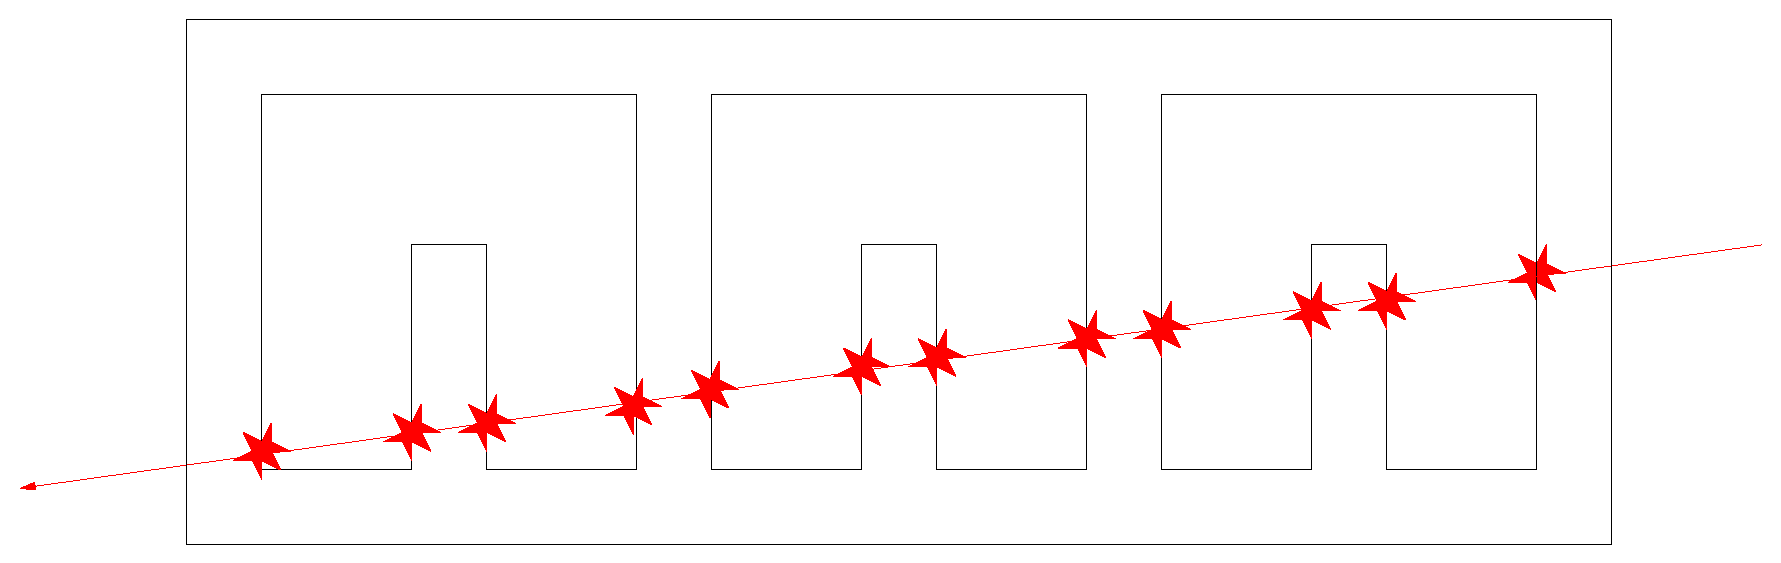
\includegraphics[width=0.6\textwidth]{Intersections}
\caption{Cartoon showing intersections of a geantino with sampled surfaces for
the GSS}
\label{fig:intersections}
\end{center}
\end{figure} 

The algorithm also requires the maximum number of possible intersections that a
line would make with the sampled volumes.  For example, Figure
\ref{fig:intersections} shows three semi-coax germanium crystals in an
enclosure.  For sampling the three crystals, the maximum number of intersections
a line would make with a sampled surface is 12.  If we were to also sample the enclosure, the
number would be 14.  To set the number of intersections, the messenger command
is

\begin{lstlisting}
 /MG/io/gss/setMaxIntersections aNumber
\end{lstlisting}

\noindent \mage \ will throw a warning if you pick a number that's too low.  Some
quick words about the efficiency of the GSS: setting the maximum number of
intersections too high will cause the GSS to unnecessarily throw away more
events, requiring a larger number of initial events to achieve the desired
number of points.  For a given number of initial events, the number of achieved
random points will vary depending on the geometry of the sampled volumes.
Sampling a sphere or pseudo-spherical assembly would be quite efficient, whereas sampling a long, thin pole would not be.

Once the desired surface points have been gathered by the GSS into a \rootv
file, it is a simple matter to use them for a physics simulation.  To read the
positions from a file, the messenger command is 

\begin{lstlisting}
 /MG/generator/gsspositionsfile GSSfilename.root
\end{lstlisting}

\noindent The GSS \rootv files will have some number of position points.  There is
an option to start at a point that is not the first one,

\begin{lstlisting}
 /MG/generator/gsseventnumber aNumber
\end{lstlisting}

\noindent but the default is to start at the beginning of the file.  If you add
more than one file, they will be chained together.


\section{Direction sampling} \label{sec:direction}
All generators but  \textsc{G4gun} sample the direction of primary particles, isotropically or 
according to specific distributions. \\

If \textsc{G4gun} is used, primary particles are shot along a given direction, 
that can be set with the macro command 
\begin{lstlisting}
 /gun/direction dx dy dz
\end{lstlisting}
It is not necessary that the components $(dx,dy,dz)$ are normalized. 
For instance, the command to generate particles directed in the negative direction 
of the z-axis is /gun/direction 0 0 $-$1. \\

Alternatively, it is possible to generate particles with direction sampled isotropically 
from a cone with given direction and given opening angle. The command to activate this 
option, which works only for the \textsc{G4Gun} generator, is
\begin{lstlisting}
 /MG/generator/g4gun/cone_on true [true] [false]
\end{lstlisting}
By default, the \texttt{cone\_on} option is set to \texttt{false} (i.e. pencil beam). 
The direction of the cone axis can be specified with the command
\begin{lstlisting}
 /MG/generator/g4gun/coneDirection dx dy dz
\end{lstlisting}
The default direction is along the positive z-axis. Similarly, the opening angle of the cone is 
set with the command
\begin{lstlisting}
 /MG/generator/g4gun/thetaDelta angle [rad/deg]
\end{lstlisting}
The default angle is 180~degrees. In this case, the direction of the primary particles is sampled 
isotropically in all the space, irrespectively of the specified direction.\\

In some applications, in order to save CPU time and optimize \mage \ performaces, it is useful to 
generate primary particles only towards the detector region. \mage \ has the
capability of sampling the direction of the primary particles only in the
direction of a given point.
This option is activated with the macro command
\begin{lstlisting}
 /MG/generator/g4gun/centric_effect_on [true] [false]
\end{lstlisting}
and the target coordinates are set using the command
\begin{lstlisting}
/MG/generator/g4gun/detector_center_position coordinates [unit]
\end{lstlisting}
Anyway, often one is not interest in a dimensionless target point, but rather in a target volume surrounding that 
point. This is necessary for instance to take into account for the extension of the real volumes and/or for changing in the 
particles direction along its propagation. There are two ways of specifying the extension of the target region 
around target point: 
\begin{enumerate}
\item the target volume is a box (default). The coordinates of the box are given with the command 
/MG/generator/g4gun/detector\_center\_position, while its dimensions along the x-, y- and z-axis are set with 
\begin{lstlisting}
/MG/generator/g4gun/detector_position_smear dimension [unit]
\end{lstlisting}
\item the direction is sampled within a cone pointing towards the target point. This option is activated 
with the command 
\begin{lstlisting}
/MG/generator/g4gun/centric_effect_cone [true] [false]
\end{lstlisting}
while the opening angle of the cone is specified by the macro command
\begin{lstlisting}
/MG/generator/g4gun/opening_angle angle [unit]
\end{lstlisting}
In this case, the direction of the cone axis depends on the initial position of the track, and it is internally 
re-calculated event-by-event.
\end{enumerate}    

\section{Energy sampling} \label{sec:energysampling}
All generators but  \textsc{G4gun} sample the energy of primary particles (e.g. cosmic ray muons, 
\textsc{Decay0}, etc.) according to their specific spectra. \\

If \textsc{G4gun} is used, primary particles are shot with a fixed kinetic energy, 
that can be set with the macro command 
\begin{lstlisting}
 /gun/energy energy [unit]
\end{lstlisting}
For instance, the command to generate 1-MeV particles is 
/gun/energy 1 MeV \\

Alternatively, it is possible to generate particles with energy spectrum sampled according 
to an histogram stored on a local file. This can be useful to generate energy spectra that 
are not provided by \textsc{Geant4}, as for instance $\beta$ spectra from forbidden transitions 
(e.g. $^{39}$Ar). In fact \textsc{Geant4} samples $\beta$ spectra according to the Fermi function, 
which is appropriate for allowed $\beta$-transitions only.
The command to activate this 
option, which works only for the \textsc{G4Gun} generator, is
\begin{lstlisting}
 /MG/generator/g4gun/spectrum_from_file [true] [false]
\end{lstlisting}
By default, the \texttt{spectrum\_from\_file} option is set to \texttt{false} (i.e. mono-energetic 
beam). \\
\emph{Notice} that energy sampling activated with the \texttt{spectrum\_from\_file} can be coupled with 
the direction sampling described in Sect~\ref{sec:direction} and the position sampling described in 
Sect.~\ref{Section:positionsampling}. For instance, it is possible to generate with \textsc{G4gun} 
primary particles emitted with a given energy spectrum (read from file), with direction in a given cone 
and with initial position distributed in a given volume. \\
% 
The file name containing the spectrum can be specified with the command
\begin{lstlisting}
 /MG/generator/g4gun/spectrum_filename [filename]
\end{lstlisting}
The information is taken into accouunt only if the flag from \texttt{spectrum\_from\_file} is set to 
\texttt{true} before the \texttt{/run/beamOn}. The program looks for the data file first in the current 
directory, and then in the directory pointed by the environment variable \texttt{MGGENERATORDATA}. Notice 
that \textsc{MaGe} will exit with an error code if one tries to run the \texttt{spectrum\_from\_file} 
option without having specified the file name and/or the data file is not found. 
The data file should have two column showing: 
\begin{lstlisting}
 energy (keV)  pdf of energy distribution (a.u.)
\end{lstlisting}

The energy spectrum does not need to be normalized, as it is re-normalized internally at the initialization 
time. The energy provided in the file should be the left edge of each bin. For the last bin, it is assumed 
that its width is equal to the width of last-but-one bin. \\

\nolinkurl{Warning}: the sampler DOES NOT interpolate inter-bin ranges. It means that the sampling will be uniform
within the binning you specify. For example, if you have 1-keV binning in the beginning, and 100-keV binning in the end,
the final distribution will have seizable steps-shape. \\

For instance, the following piece of macro generates $^{39}$Ar $\beta$ decays, with energy spectrum read 
from the file \texttt{ar39.dat} and isotropic angular distribution:
\begin{lstlisting}
 /MG/generator/select G4gun
#
# Here set the energy sampling from ar39.dat
#
 /MG/generator/g4gun/spectrum_from_file true
 /MG/generator/g4gun/spectrum_filename ar39.dat
#
# Get isotopic particles. By default the axis of the cone is
# the z-axis, with 180 deg opening angle (= isotropic)
#
 /MG/generator/g4gun/cone_on true
#
\end{lstlisting}

\section{TUNL Generator}
%FixME section owned by Reyco

\section{Wang Neutron Generator}
%FixME section owned by Reyco



\chapter{Geometries}
\label{chapter:geometries}

\section{Common Geometries}

\subsection{Geometry From File}
To switch on the geometry definition from an external file, the messenger 
command 
\begin{lstlisting}
/MG/geometry/detector GeometryFile
\end{lstlisting}
has to be given. The name of the file containing the geometry to be read 
is set using the command 
\begin{lstlisting}
/MG/geometry/geometryFileName mygeometry.def
\end{lstlisting}
If the command \texttt{/MG/geometry/geometryFileName} is issued more than 
once, the file name is overwritten, and the last one is taken into account. 
If the general geometry has not been set with the command 
\texttt{/MG/geometry/detector GeometryFile}, the file name is anyway accepted 
but it is not used. If the file name is not given explicitly, the default 
\texttt{geometry.def} is looked for in the current directory. \\
It is possible to define an arbitrary 
number of boxes, cylinders and spheres. Volumes can be daughters of the 
world or of an other volume. In the latter case, it is possible to define 
``holes'' in a given volume. \\
An example of geometry definition file is the following: \\
\begin{lstlisting}
1 Crystal 2 1 0 SodiumIodide   
0. 0. 2.55 
2.55 5.10 0. 
0. 0. 0. 
2 Hole    2 0 1 Air             
0. 0. 0.65 
1.43 3.80 0.
0. 0. 0. 
\end{lstlisting}
Each volume is defined in four lines. \\
(1) The entries for the first line are:
\begin{itemize}
\item ordering number (int).
\item volume name (string). This is the name of the physical volume defined 
in the geometry. It can be used, for instance, for the uniform sampling 
routine. The names of the volumes should be different, though there is no 
specific control in the program. 
\item shape of the volume (int). The code is 1 for boxes, 2 for cylinders and 
3 for spheres. If the code is different from the values listed above, the volume  
is ignored.
\item sensitive detector flag (int). If the flag is 1, the volume is 
registered as a sensitive detector for the subsequent analysis. 
\item mother flag (int). If the flag is set to 0, the volume is placed inside the 
world volume. If the flag is a non-zero integer $n$, the volume is considered 
to be a daughter of the volume $n$. The mother volume must be defined 
\emph{before} the daughter one (namely, the ordering number of the Daugherty 
must be larger than $n$). It is possible to nest daughter volumes one inside 
the other.
\item material name. The material has to be included in the \mage database 
or defined using an external file, as described in Sect.~\ref{subsection:materials}.
\end{itemize}
(2) The second line contains the three coordinates of the volume center, given in cm (double). 
Coordinates are always expressed with respect to the mother volume reference system. \\
(3) The third line contains the three physical dimensions of the volume (double), given in cm. 
For boxes, the numbers are the sizes along the $x$, $y$ and $z$ axes, respectively. 
For cylinders, the first parameter is the radius, and the second the height (the 
third parameter is unused).  
For spheres, the first parameter is the radius, the other two are unused. \\
(4) The fourth line contains the three Euler angles (degrees) defining the volume rotation. 
The angles are always referred to the mother volume reference system. \\
The volumes defined in the external file are placed in a world volume made of air. The 
world volume is a cube of 5~m size. Therefore, the dimensions of the volumes in 
the file cannot exceed 5~m.\\
The geometry file presented above represents: a cylindrical sodium iodide detector (radius 
2.55~cm, height 5.10~cm) with a cylindrical hole (radius 1.43~cm, height 3.8~cm) displaced 
of 0.65~cm along the $z$-coordinate of the detector. The coordinates of the center of the 
detector are (0,0,2.55~cm) with respect to the world reference frame. The sketch of the 
geometry is displayed in Fig.~\ref{testgeometry}. \\
%%
\nopagebreak
\begin{figure}[tb]
\begin{center}
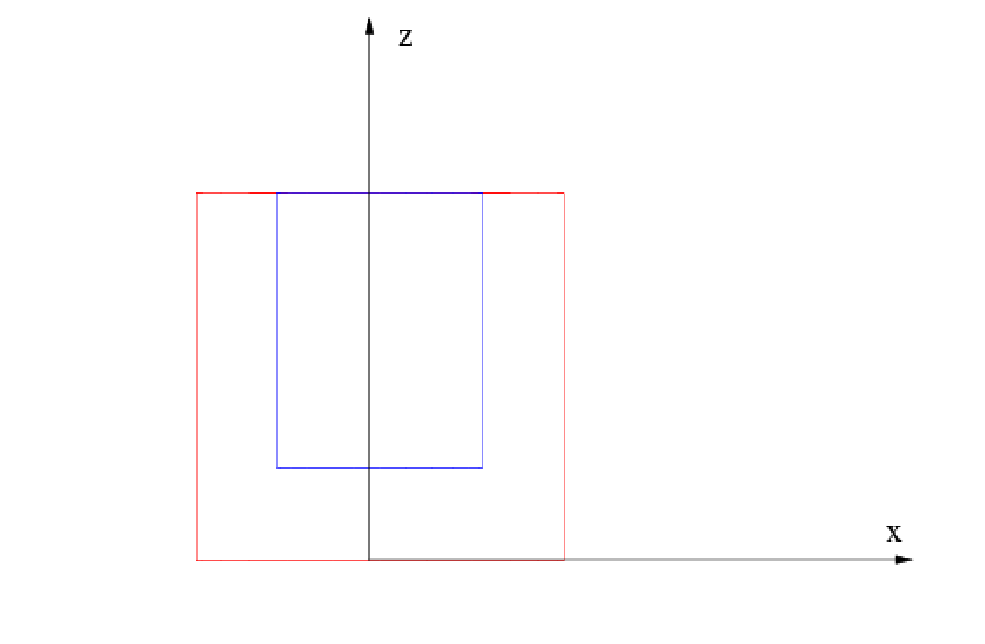
\includegraphics[height=10cm]{figures/geom-from-file}
\caption{Sketch of the setup geometry defined in \textsc{MaGe} with the external 
data files used as example in the text.}\label{testgeometry}
\end{center}
\end{figure}
%
\section{GERDA Geometries}
 
\subsection{GERDA Phase I}
\begin{lstlisting}
/MG/geometry/detector GerdaArray
/MG/geometry/detector/geometryfile geometry.dat
/MG/geometry/detector/matrixfile matrix_phase_i.dat
\end{lstlisting}
The standard GERDA setup (to be specified) including the detector
array (with cables and holders), the cooling liquid (argon), the
cryogenic tank, the water tank, the lock and the cleanroom. Also
included are the PMTs and the plastic scintillator on top of the
cleanroom. Parts of the infrastructure, in particular beams between
the cleanroom and the water tank, are also simulated. The detectors
are described in geometry.dat, the array configuration is described in
matrix\_phase\_xxx.dat\\

The Phase~I setup includes an array of 9 non-true coaxial
detectors. They are stacked in three strings of three detectors each.

\subsection{GERDA Phase II}
\begin{lstlisting}
/MG/geometry/detector GerdaArray
/MG/geometry/detector/geometryfile geometry.dat
/MG/geometry/detector/matrixfile matrix_phase_ii.dat
\end{lstlisting}

See GERDA Phase~I for the general setup. The Phase~II setup includes
five true coaxial and three non-true coaxial detectors per layer for
three layers in total. 

\subsection{GERDA Phase II Ideal}
\begin{lstlisting}
/MG/geometry/detector GerdaArray
/MG/geometry/detector/geometryfile geometry.dat
/MG/geometry/detector/matrixfile matrix_phase_ii_ideal.dat
\end{lstlisting}

See GERDA Phase~I for the general setup. The Phase~II ideal setup
includes seven true coaxial detectors per layer for three layers in
total.

\subsection{Test Stand Simple}
\begin{lstlisting}
/MG/geometry/detector MunichTestStand
/MG/geometry/teststand/teststandtype simple
\end{lstlisting}

Describes a ReGe detector with a source placed infront of it. The
source is surrounded by lead bricks. The distance between the crystal
and the source as well the distance between the source and the lead
bricks can be set by macro with
\verb*|/MG/geometry/teststand/crystaltosource| and
\verb*|/MG/geometry/teststand/sourcetobrick|, respectively. 

%\subsubsection{Test Stand Siegfried}
%FixME Jing
%\begin{lstlisting}
%/MG/geometry/detector MunichTestStand
%/MG/geometry/teststand/teststandtype siegfried
%\end{lstlisting}

\subsection{Test Stand LN2}
\begin{lstlisting}
/MG/geometry/detector MunichTestStand
/MG/geometry/teststand/teststandtype ln2
\end{lstlisting}

Simulates an unsegmented DSG p-type detector in the GERDAlinchen test
stand, i.e. a cryostat filled with liquid nitrogen. It includes an AEA
source inside the cryogenic liquid. 

\subsection{Heidelberg Detectors}
\begin{lstlisting}
/MG/geometry/detector Bruno
/MG/geometry/detector Corrado
/MG/geometry/detector Dario
\end{lstlisting}

Simulates the three main detectors used at Heidelberg for material screening.
Includes full models of shielding and samples. The samples can be defined
by the following command:
\begin{lstlisting}
/MG/geometry/dario/sample [sphere] [box] [tube] [sbox] [liquid] [twobox]
[marinelli] [custom]
\end{lstlisting}
For different detectors replace the detector name in the command (and all following commands) accordingly, e.g. for Bruno : \texttt{/MG/geometry/bruno/sample}.\\
Description of sample options :\\
(1) The default geometry option is \texttt{sphere}, which creates a sphere of fixed radius 0.1 $\mu$m. This is used only to put the volume \texttt{sample} out of way when generating gammas from a single point.\\
(2) The outer dimensions of geometry \texttt{box} can be set by the following self-explanatory commands:
\begin{lstlisting}
/MG/geometry/dario/boxwidth dimension [unit]
/MG/geometry/dario/boxheight dimension [unit]
/MG/geometry/dario/boxthickness dimension [unit]
\end{lstlisting}
(3) The geometry \texttt{tube} produces a cylinder with a possible concentric hole. The dimensions can be specified by the following parameters:
\begin{lstlisting}
/MG/geometry/dario/tubelength dimension [unit]
/MG/geometry/dario/tubeouterradius dimension [unit]
/MG/geometry/dario/tubeinnerradius dimension [unit]
\end{lstlisting}
(4) The geometry \texttt{sbox} is identical to \texttt{tube} (the same dimension-parameters apply), but adds a standard cylindrical
box used for measurements at MPIK laboratory (lid facing the detector). The position of the container changes according to the position of the sample, but the size is fixed, so it's users responsibility to ensure the \texttt{sample} volume fits inside and doesn't overlap with the container volume. The default dimensions of the sample cylinder correspond to the inner dimensions of the standard cylindrical box, so for samples which fill the inner volume completely, these parameters don't need to be specified.\\
(5) The geometry \texttt{liquid} is an extension of the \texttt{sbox} geometry. It subtracts a flat volume from the top of the sample, to simulate liquid not filling completely the volume of the standard box. For defining the liquid level, the command \texttt{/MG/geometry/dario/boxheight} is used. The value corresponds to liquid level measured from top (vertical dimension of the missing part).\\
(6) The geometry \texttt{twobox} adds two (empty) standard cylindrical containers in front of the detector.\\
(7) The geometry \texttt{marinelli} (not available for \texttt{Bruno} detector) is an extension of the \texttt{sbox} geometry. It creates a marinelli shaped sample (a box with a hole), with external dimensions defined by \texttt{boxwidth}, \texttt{boxheight} and \texttt{boxthickness} parameters, and internal hole depth and radius defined by \texttt{tubelength} and \texttt{tubeouterradius} parameters. The parameter \texttt{tubeinnerradius} is used to displace the hole from the center in vertical direction.\\
(8) The option \texttt{custom} selects additional geometry, which can't be described by previous commands, but has to be coded in the detector construction source file.\\
The following parameters define the sample position with respect to the center of the front 
detector window :
\begin{lstlisting}
/MG/geometry/dario/samplexpos dimension [unit]
/MG/geometry/dario/sampleypos dimension [unit]
/MG/geometry/dario/samplezpos dimension [unit]
\end{lstlisting}
The command:
\begin{lstlisting}
/MG/geometry/dario/samplematerial [material name]
\end{lstlisting}
defines the material of the sample. A material with the same name has to be defined in \texttt{MGGerdaLocalMaterialTable.cc} or from external file with the \texttt{/MG/geometry/addMaterial} command, as described in Sect.~\ref{subsection:materials}.\\
Additional commands can be used with detector \texttt{Dario} to adjust the parameters of the crystal:
\begin{lstlisting}
/MG/geometry/dario/detzpos dimension [unit]
\end{lstlisting}
Guidance: Sets the distance in \texttt{z} direction between the detector window and crystal surface.
\begin{lstlisting}
/MG/geometry/dario/deadthickness dimension [unit]
\end{lstlisting}
Guidance: Sets the dead layer thickness.
\begin{lstlisting}
/MG/geometry/dario/detdiameter dimension [unit]
\end{lstlisting}
Guidance: Sets outer diameter of the crystal (including dead layer).
\begin{lstlisting}
/MG/geometry/dario/detlenght dimension [unit]
\end{lstlisting}
Guidance: Sets lenght of the crystal (including dead layer).

\section{Majorana Geometries}

\subsection{17-A}
% FixME Rob J.
\begin{lstlisting}
/MG/geometry/detector MJ17A
\end{lstlisting}

\subsection{57-Banger}
% FixME Reyco
\begin{lstlisting}
/MG/geometry/detector MJ57Banger
\end{lstlisting}

\subsection{CERN NA55 Experiment}
% FixME mgm
\begin{lstlisting}
/MG/geometry/detector CERN_NA55
\end{lstlisting}
This geometry describes an experiment performed at CERN in which neutrons
produced from a 190~GeV muon beam incident on various beam stops were
measured.  The geometry consists of a (selectable) beam stop and a bounding
sphere.  For more information on the experiment, please see 
V.~Chazal et al., Nucl.~Inst.~Meth.~Phys.~Res.~A 490, p 334-343 (2002)
\subsubsection{Options}
\begin{enumerate}
\item 
\begin{lstlisting}
/MG/geometry/CERN_NA55/setBeamDumpType [Graphite] [Copper] [Lead]
\end{lstlisting}
Guidance: Set type of beam dump.
\end{enumerate}

\subsection{Clover Detectors}
% FixME Alexis/Reyco/Kareem
\begin{lstlisting}
/MG/geometry/detector [clover] [cloverinNaIbarrel] [cloverInShield]
\end{lstlisting}
The clover geometry models the Canberra clover detector, which  consists 
of four n-type Ge crystals. The "clover" option is the basic clover detector.
The "cloverinNaIbarrel" option produces the clover detector in an NaI veto 
barrel used for TUNL FEL testing.  The "cloverInShield" option is based on an 
experiment performed at LANL, and produces the basic clover detector in a lead 
shield, with a polyethylene moderator between the shield and detector on one 
side, as used in an experiment at LANL.  The experiment at LANL used an 
americium beryllium source, and the "cloverInShield" detector includes an 
option to create a housing for the source.  If the housing is used, its 
position must be specified.  

\subsubsection{Clover In Shield Options}
\begin{enumerate}
\item 
\begin{lstlisting}
/MG/geometry/cloverInShield/moderatorThickness [dimension with units of length] 
\end{lstlisting}
Guidance: Set thickness of moderator.
\item 
\begin{lstlisting}
/MG/geometry/cloverInShield/shieldThickness [dimension with units of length] 
\end{lstlisting}
Guidance: Set thickness of lead shield.
\item 
\begin{lstlisting}
/MG/geometry/cloverInShield/useAmBeHousing [true] [false] 
\end{lstlisting}
Guidance: Select whether to use housing for the AmBe generator.
\item 
\begin{lstlisting}
/MG/geometry/AmBeHousing/position [x y z units of length]
\end{lstlisting}
Guidance: Set location of center of housing, which should match source position.
\end{enumerate}

\subsection{Ideal Coaxial Crystal in a Shield}
% FixME Reyco
\begin{lstlisting}
/MG/geometry/detector idealCoax
\end{lstlisting}

\subsection{MJ LArGe}
% FixME Reyco, Marie DiMarco
\begin{lstlisting}
/MG/geometry/detector LArGe
\end{lstlisting}

\subsection{LLNL Detector}
% FixME Reyco
\begin{lstlisting}
/MG/geometry/detector LLNL8x5
\end{lstlisting}

\subsection{MEGA cryostat}
% Alexis
\begin{lstlisting}
/MG/geometry/detector MJMEGA
\end{lstlisting}
This geometry models an experiment at the Waste Isolation Pilot Plant (WIPP) in
Carlsbad, New Mexico.  The geometry consists of an annular copper cryostat, 
and four identical Ge crystals arranged in two two-crystal stacks.  The 
cryostat is surrounded by a lead shield.  This geometry uses the Ideal Coax Crystal class.  Dimensions and properties of the crystals should be specified with 
options for the Ideal Coax Crystal class.

\subsection{MJ Reference Design Detectors}
% FixME Reyco
\begin{lstlisting}
/MG/geometry/detector [MJRDBasicShield] [MJRDCryostat] [MJRDCrystalColumn]
\end{lstlisting}

\subsection{SLAC Beam Dump Experiment}
% FixME mgm 
\begin{lstlisting}
/MG/geometry/detector SLACBD
\end{lstlisting}
This geometry models an electron beam experiment that took place at SLAC.  (Please
see S.~Taniguchi et al., Nucl.~Inst.~Meth.~Phys.~Res.~A 503, p 595 (2003) and 
S.~Roesler et al., Nucl.~Inst.~Meth.~Phys.~Res.~A 503, p 606 (2003) for information 
on the experiment.) The geometry consists of an aluminum beam dump surrounded by a steel and concrete shield.  
This geometry has been used to model and validate neutron propagation.
\subsubsection{Options}
\begin{enumerate}
\item 
\begin{lstlisting}
Command /MG/geometry/SLACBD/setShieldThickness [None] [Thin] [Medium] [Thick]
\end{lstlisting}
Guidance : Set thickness of concrete shield.

\end{enumerate}

\subsection{Solid Block}
% FixME Reyco 
\begin{lstlisting}
/MG/geometry/detector solidBlock
\end{lstlisting}

\subsection{UW LArGe}
% FixME J. Orrell, Reyco 
\begin{lstlisting}
/MG/geometry/detector UWLArGe
\end{lstlisting}

\subsection{WIPPn}
% FixME Rob J.  
\begin{lstlisting}
/MG/geometry/detector WIPPn
\end{lstlisting}


% -------------------------------------------------------- 
% analysis tools
% --------------------------------------------------------  

\chapter{Analysis tools} 
\label{chapter:tools} 
{\it Xiang} 
\section{Handling of decay chains} 

Radioactive decay in \geant \ is handled by the radioactive decay module(RDM).
The RDM will handle an entire decay chain, including proper branching ratios.
The chain all happens in one \geant \ event, so it is up to the user to divvy up
the chain into events that a physical detector would actually measure.  One way
of doing this is to keep track of each particle's global time.  The global time
of a track in \geant \ is the time since the track was created({\tt
aTrack$\rightarrow$GetGlobalTime()}).   Steps of an event that fall within a
user-prescribed window of time are then gathered together.  The time window
would typically correspond to the time resolution of the DAQ.  The user's output
class would then write to a \rootv \ object more often than once a \geant \ event.  

A problem arises because of the finite precision of a double.  In decimal form,
a G4double is only accurate to 15 digits or so.  Following the decay of
$^{238}$U, the global time of the daughter nucleus, $^{234}$Th would be on the
order of 5 $\times 10^9$ years, or $10^{17}$ seconds.  Each additional decay
only adds more to the global time.  If one wishes to gather steps that fall
within a typical time window of say, 15 $\mu$s, then one must find steps that
differ in time by $\sim$ 1 part in $10^{22}$.  This is treated as zero.

The workaround to this involves resetting the GlobalTime of a track that was
spawned by radioactive decay to zero if it is too large.  Any comparison of
global times can then yield the desired sensitivity.  A new variable, {\tt
fOffsetTime} is kept separate from GlobalTime, and is incremented to keep track
of the actual global time.

\subsection{Stacking Actions}

A brief comment on stacking actions.  When a track is created by a process, it
is sent to any UserStackingAction that is in place.  In \mage, the
UserStackingAction resides in the output classes that derive from {\tt
MGVOutputManager}.  The StackingAction can look at the track and determine
whether to put it in the ``Urgent" stack or the ``Waiting" stack.  When all
tracks in the urgent stack are finished, then all tracks in the waiting stacks
are transferred(all at once) to the urgent stack.  The urgent stack is then
processed as normal by \geant.  The StackingAction allows for a user-defined
{\tt NewStage()} function that is called once all tracks in the urgent stack are
finished.

\subsection{TimeWindower Implementation}

The UserStackingAction set in MaGe.cc is {\tt MGManagementStackingAction}.  It
has three functions, {\tt ClassifyNewTrack(const *G4Track)}, {\tt NewStage()},
and {\tt PrepareNewEvent()}.  These functions call their corresponding
counterparts in whatever output class you use that derives from {\tt
MGVOutputManager}.  One note of possible confusion, the {\tt
ClassifyNewTrack(const *G4Track)} points to output function {\tt
StackingAction(const *G4Track)} in the output class.  The {\tt
StackingAction(const *G4Track)} and the {\tt NewStage()} functions are written
in {\tt MGVOutputManager} and probably don't need to be messed with unless
you're doing something complicated.  The {\tt MGVOutputManager} also defines a
{\tt WritePartialEvent(const *G4Event)} and {\tt ResetPartialEvent(const
*G4Event)} functions.  Each individual output class needs to have its own
version of these two functions to properly use the TimeWindower.

The use of time windowing is specified by macro(default is off), as is the actual window of time to use.
If the macro specifies time windowing, then the {\tt StackingAction(const
*G4Track)} looks at each track as it is created.  If the creator process was
RadioactiveDecay and the GlobalTime is larger than the time window, then:

\begin{itemize}
\item the track's global time is stored
\item the track's global time is set to zero
\item the track is given the ``waiting" classification, so it is sent to the waiting stack
\end{itemize}

If all tracks in the urgent stack have been processed and there are tracks in
the waiting stack, then {\tt NewStage()} is called.  The {\tt fOffsetTime} is
updated, and {\tt WritePartialEvent(const *G4Event)} and {\tt
ResetPartialEvent(const *G4Event)} are called.  These functions obviously
depends on the output class being used, but the general idea is that the event
is written to a \rootv \ file, and any necessary arrays/variables/etc... are reset.
Only after all this are the tracks in the waiting stack sent to the urgent
stack.  It's worth mentioning that {\tt NewStage()} only happens if there are
tracks in the waiting stack.  If not, then the output class's {\tt
EndOfEventAction()} should handle the end of the actual \geant \ event.


\subsection{How to use the TimeWindower}

First, make sure that the WritePartialEvent() and ResetPartialEvent() functions have been implemented in your 
output class(look at the {\tt MGOutputG4Steps} class for an example of how to do
this).  You will also need to add messenger commands to your output messenger
class.  You can handle everything by messenger in a macro.  The macro commands
are:

{\tt
/MG/io/G4Steps/useTimeWindow

/MG/io/G4Steps/setTimeWindow
}

\noindent Where you would substitute your output class for G4Steps.

%\end{document}  





% -------------------------------------------------------- 
% part ii
% -------------------------------------------------------- 

\part{Developer's guide} 
\label{part:developer} 

% -------------------------------------------------------- 
% compiling
% --------------------------------------------------------  

\chapter{Compiling \mage} 
\label{chapter:compiling} 
% {\it Jing} 
\input{compiling.tex}

% -------------------------------------------------------- 
% code structure
% --------------------------------------------------------  

\chapter{\mage~Code Structure} 
\label{chapter:codestructure} 
\section{Introduction }

The simulation package is written in C++ and uses object-{}oriented
         programming techniques and the STL. 
         The geometry, tracking and physics package
         is Geant 4 based. A working knowledge of Geant 4 is required to 
         follow the discussions in this section. 
         Waveform simulation is performed with custom software.
 

\section{Program Structure}

       The program consists of sets of C++ classes that are grouped into
      software packages. All the software packages are built into a 
      single executable, \nolinkurl{MaGe}. The simulation is 
      setup by selecting detector geometries,
      physics processes, generators, etc. via text macros based on Geant 4 
      messengers. The software packages name's, with their corresponding CVS
      directory names in brackets, are given below: 
 

\begin{lstlisting}
  MaGe--
     |- Database (database)
     |- Generators (generators)
     |- Geometry (geometry)
     |- Gerda specific geometry (gerdageometry)
     |- Majorana specific geometry (mjgeometry)
     |- Output (io)
     |- Gerda specific output (gerdaio)
     |- Majorana specific output (mjio)
     |- Management (management)
     |- Materials (materials)
     |- Processes (processes)
     |- Waveform (waveform)
   \end{lstlisting}

      Note that not every CVS directory contains a software package, since 
     some CVS directories, ie. \nolinkurl{doc}, do not contain
     parts of the simulation program. Other packages, such as 
 \nolinkurl{Geometry}, are spread over several CVS directories
     to separate code from the Gerda and Majorana.  
     Each package is discussed in detail in subsequent chapters. We will give
     a brief summary of each package here, as well as how they are connected.
 

\noindent
\begin{description}
\item[{Database}] 

             Interfaces with the PostGreSQL database server.
            The database is used to store geometry data and calibration 
            constants and also contains all the materials definitions.
	    Currently only used by the Majorana experiment.
 


\item[{Generators}] 

             The different event generators. Currently several event
	    generators are supported and are user-{}selectable at runtime. See
 Chapter \ref{Physics}.
 


\item[{Geometry}] 

             The classes describing the different detector geometries. 
            It is possible to combine different geometries into a single 
            detector, ie. a NaI veto barrel around a clover detector, the
	    Gerda detector geoemetry, etc. 
            See Chapter \ref{Geometry}.
 


\item[{Output}] 

          The classes describing the different output for the 
         different detectors. Both AIDA and Root are supported. 
	 It is possible to have more than one output class
         per detector. 
	 Also contains the \nolinkurl{MGLogger} class 
         that handles terminal
         output and error messages. See Chapter \ref{IO}  


\item[{Management}] 

 	   Management classes, including 
 \nolinkurl{MaGe/management/MaGe.cc} that contains the 
 \texttt{m\-a\-i\-n\-(\-)}. See 
 Section \ref{Structure_Implement} for more information on the 
           management 
           classes.
 


\item[{Materials}] 

            These classes automatically build requested materials from elements
           that are in turn build from isotopes. All material, elemental and
           isotopic data are stored in the database. All new materials
           have to be added to the database. See Chapter \ref{Geometry}  


\item[{Processes}] 

            User-{}selectable Geant 4 physics lists for specific simulations, ie. 
           double-{}beta decay studies requires different physics process than
           dark matter studies. See Chapter \ref{Physics}.
 


\item[{Waveform}] 

            Waveform simulation package. Can be run independently from Geant 4. 
           Not yet implemented. See Chapter \ref{Waveforms}.
 



\end{description}

\section{How Everything is Implemented and 
Fits Together.}
\label{Structure_Implement}

       In the \nolinkurl{main()} function a collection
      of ``management" classes are instantiated. These classes control specific
      components of the framework. Classes can communicate with each other
      via the singleton \nolinkurl{MGManager} class. The 
 \nolinkurl{MGManager} class is instantiated 
      in the file \nolinkurl{MG/management/MaGe.cc}, and is 
      a collection of pointers to all the management classes.
      By using the \nolinkurl{MGManager} class, global variables are
      avoided.  
 

       The management class are listed below in the order they are instantiated:
 

\noindent
\begin{description}
\item[{\nolinkurl{MGGeometryDetectorConstruction}}] 

          Selects detector geometry via Geant 4 messenger and constructs it
         in Geant 4. Also constructs all required materials from the database,
	 if requested by the selected detector.
         See Chapter \ref{Geometry}. Accessed via:
 \texttt{M\-G\-M\-a\-n\-a\-g\-e\-r\-:\-:\-G\-e\-t\-M\-G\-G\-e\-o\-m\-e\-t\-r\-y\-D\-e\-t\-e\-c\-t\-o\-r\-C\-o\-n\-s\-t\-r\-u\-c\-t\-i\-o\-n\-(\-)}  


\item[{\nolinkurl{MGProcessesList}}] 

          Geant 4 physics list. User can select different physics packages
         via Geant 4 messengers. See Chapter \ref{Physics}. Accessed via:
 \texttt{M\-G\-M\-a\-n\-a\-g\-e\-r\-:\-:\-G\-e\-t\-M\-G\-P\-r\-o\-c\-e\-s\-s\-e\-s\-L\-i\-s\-t\-(\-)}  


\item[{\nolinkurl{MGManagementVisualization}}] 

          Registers Geant 4 visualization packages. Performs no other actions.
 


\item[{\nolinkurl{MGGeneratorPrimary}}] 

          Selects and manages event generators. See Chapter \ref{Physics}.
	 Accessed via:
 \texttt{M\-G\-M\-a\-n\-a\-g\-e\-r\-:\-:\-G\-e\-t\-M\-G\-G\-e\-n\-e\-r\-a\-t\-o\-r\-P\-r\-i\-m\-a\-r\-y\-(\-)}  


\item[{\nolinkurl{MGManagementRunAction}}] 

          Performs pre-{} and post run actions by 
         executing \texttt{B\-e\-g\-i\-n\-O\-f\-R\-u\-n\-A\-c\-t\-i\-o\-n\-(\-)} 	 and \texttt{E\-n\-d\-O\-f\-R\-u\-n\-A\-c\-t\-i\-o\-n\-(\-)} methods 
         of output
         classes. Derived from \nolinkurl{G4UserRunAction}.
	 Accessed via:
 \texttt{M\-G\-M\-a\-n\-a\-g\-e\-r\-:\-:\-G\-e\-t\-M\-G\-R\-u\-n\-A\-c\-t\-i\-o\-n\-(\-)}  


\item[{\nolinkurl{MGManagementEventAction}}] 

          Performs pre-{} and post event actions by 
         Executing \texttt{B\-e\-g\-i\-n\-O\-f\-E\-v\-e\-n\-t\-A\-c\-t\-i\-o\-n\-(\-)} 	 and \texttt{E\-n\-d\-O\-f\-E\-v\-e\-n\-t\-A\-c\-t\-i\-o\-n\-(\-)} methods 
         of output
         classes. Selects and contains pointer to Root output class 
         (Chapter \ref{IO}). 
         Derived from \nolinkurl{G4UserEventAction}.
	 Accessed via:
 \texttt{M\-G\-M\-a\-n\-a\-g\-e\-r\-:\-:\-G\-e\-t\-M\-G\-E\-v\-e\-n\-t\-A\-c\-t\-i\-o\-n\-(\-)}  


\item[{\nolinkurl{MGManagementSteppingAction}}] 

          Performs actions during each step of Geant 4 tracking by  
         executing \texttt{U\-s\-e\-r\-S\-t\-e\-p\-p\-i\-n\-g\-A\-c\-t\-i\-o\-n\-(\-)}          method of root output classes.
	 Derived from \nolinkurl{G4UserSteppingAction}.
	 Accessed via:
 \texttt{M\-G\-M\-a\-n\-a\-g\-e\-r\-:\-:\-G\-e\-t\-M\-G\-S\-t\-e\-p\-p\-i\-n\-g\-A\-c\-t\-i\-o\-n\-(\-)}  



\end{description}

       A pointer to the \texttt{M\-G\-M\-a\-n\-a\-g\-e\-r} singleton 
      class is accessible via the 
 \texttt{M\-G\-M\-a\-n\-a\-g\-e\-r\-:\-:\-G\-e\-t\-M\-G\-M\-a\-n\-a\-g\-e\-r\-(\-)} method.
      The Geant 4 visualization and run manager are also accessible via:
 \texttt{M\-G\-M\-a\-n\-a\-g\-e\-r\-:\-:\-G\-e\-t\-G\-4\-R\-u\-n\-M\-a\-n\-a\-g\-e\-r\-(\-)} and
 \texttt{M\-G\-M\-a\-n\-a\-g\-e\-r\-:\-:\-G\-e\-t\-G\-4\-V\-i\-s\-M\-a\-n\-a\-g\-e\-r\-(\-)} methods.
 

       There are two packages that are not accessible via the 
 \texttt{M\-G\-M\-a\-n\-a\-g\-e\-r}. The first is the Waveform
      package that is not implemented yet. It will be accessible via 
 \texttt{M\-G\-M\-a\-n\-a\-g\-e\-r} when it is implemented. 
      The other
      is the database. For historical reasons, it is accessed via it's own
      singleton control class: \texttt{M\-G\-D\-a\-t\-a\-b\-a\-s\-e}. See
 Chapter \ref{Database}.
 

\section{Programming Guidelines and Naming Conventions}

   MaGe requires the use of good object-{}oriented programming techniques.
  We strongly discourage the use of ``Fortranized" C++. Our coding conventions
  are based on modified  
 \href{http://root.cern.ch/root/Conventions.html}{Root} and 
 \href{http://pcroot.cern.ch/TaligentDocs/TaligentOnline/DocumentRoot/1.0/Docs/books/WM/WM_3.html}{   Taligent guides }. Enforcing too rigid 
  programming rules are not feasible, although we require the following 
  reasonable conventions:
 
\begin{itemize}

\item{}           All class names begin with \texttt{G\-E\-, M\-G},
	  or \texttt{M\-G}. 
 \texttt{G\-E} is reserved for classes specific
	  to the Gerda simulation, such as geometries. 
 \texttt{M\-J} is specfically for Majorana 
	  classes. Common classes, such as management, start with 
 \texttt{M\-G}. If in doubt, use 
 \texttt{M\-G}.
 


\item{}           All virtual base class names begin with 
 \texttt{M\-G\-V\-, M\-G\-V\-, G\-E\-V}.
 


\item{}           All class member variables names begin with 
 \texttt{f}  


\item{}           All local automatic variables names must begin with a lowercase, ie 
 \texttt{s\-o\-m\-e\-L\-o\-c\-a\-l\-R\-a\-n\-d\-o\-m\-N\-u\-m\-b\-e\-r}  


\item{}          All variable, class names, etc. should have descriptive, 
         written out names. Think carefully about naming and avoid ambiguity.
 


\item{}          All unitialized pointers should be set to 0 or 
 \texttt{N\-U\-L\-L}.
 


\item{}          All terminal output should be done via the 
 \nolinkurl{MGLogger} class, if possible. 
	 See Section \ref{IO_MGLogger}. 
 


\item{}          Code should be indented 3 spaces per nesting level. 
 


\item{}          Lines longer than 80 columns should be wrapped with a carriage return.
 


\item{}          The use of a separator between methods, ie.
 

\begin{lstlisting}
//---------------------------------------------------------------------------//
\end{lstlisting}

          is strongly encouraged.
 

\end{itemize}

    Some of the older code in the \nolinkurl{MaGe}    package do not follow these rules, since they were written before the rules 
   were made explicit. Please do not follow their conventions. If you 
   encounter any cases not covered here, use the Root/Taligent guideline, 
   use you best judgment, or contact Reyco Henning (Majorana) or 
   Xiang Liu (Gerda).
 
%\begin{DBKadmonition}{warning}{Important}
% FixME there should be some sort of admonition added here
\emph{Remember that you are not coding for yourself! Many others will have to read you code. Write the code the way you would like to read it!}  
%\end{DBKadmonition}




% -------------------------------------------------------- 
% physics lists  
% --------------------------------------------------------  

\chapter{Physics lists}
\label{chapter:physics}
{\it Luciano} \\ 
\section{Introduction}

This section gives a high-level description of the physics list used
in the MaGe framework, and documents the MGProcesses Messenger that
provides a small amount of user control over that list. All macro commands 
relative to physics list must be issued in the \texttt{Pre\_init} phase, 
namely before the \texttt{/run/initialize}. 
 
\section{MGProcesses description}
The MaGe framework physics list is an amalamation of two physics lists
that are distributed with the GEANT4 simulation package. One part of
the list comes from the list included as part of the Underground
Physics advanced example. The other part of the list comes from the
QGSP\_HP hadronic list. Documentation on these lists are available on
the GEANT4 website. It manages the processes for Optical Photons 
(Cherenkov emission, Scintillation, Absorption) supports the cut-per-region 
approach: this allows to set different production cuts in different regions 
of the geometry.

The primary class is the MGProcessesList class, but it uses
supporting classes MGProcessesMaxTimeCuts, MGProcessesMinEkineCuts,
and MGProcessesSpecialCuts.

\section{Details of the physics lists}
\subsection{Interactions of hadrons}
The hadronic part of the physics list (default) is composed by 
\begin{enumerate}
\item theory-driven quark-gluon string models (QGSP) for the energetic pions, kaons, and nucleons, 
up to 100~TeV; 
\item LEP parametrized models for inelastic interactions of pions and nucleons below 25~GeV;
\item tabulated cross-section data derived from the 
ENDF/B-VI database to model capture, fission elastic scattering and 
inelastic scattering of neutrons from thermal energies up to 20~MeV (HP models). 
\end{enumerate}
%
Alternatively, the physics list developed by M.~Bauer (QGSP\_GN\_HP\_BIC\_ISO) for the description 
of muon-induced neutron production can be used. The list is chosen using the macro command
\begin{lstlisting}
 /MG/processes/qgsp_hadron_list true
\end{lstlisting}
The main difference with respect to the default physics list is that Binary cascade models (BIC) 
are used insted of LEP parametrized models for the 
description of nucleon and pion interactions below 10~GeV. It is also possible to replace the 
Binary cascade models with the Bertini (BERT) cascade models for the same energy range. 
The macro command is
\begin{lstlisting}
 /MG/processes/useBertCascade true
\end{lstlisting}
If the physics list is set to M.~Bauer's one , the quark-gluon plasma string 
model (QGSP) 
for the description of high-energy interactions can be replaced with chiral-invariant-phase-space 
models (CHIPS) for the de-excitation for the quark-gluon plasma. The macro command is 
\begin{lstlisting}
 /MG/processes/useQGSC true
\end{lstlisting}
As specified above, the latter command works only after
\begin{lstlisting}
 /MG/processes/qgsp_hadron_list true
\end{lstlisting}
%
For some applications, it may be useful to switch off all the hadronic interactions. It is 
possible in MaGe with the command 
\begin{lstlisting}
 /MG/processes/useNoHadPhysics true
\end{lstlisting}
In this case, all the additional specifiers described avove (e.g. useBertCascade or useQGSC) have no 
effect.
%
\subsection{Interactions of electrons, positrons and $\gamma$-rays}
The specific low-energy \geant\ models~\cite{geant4physics} are used by default for the description 
of the electromagnetic interactions of $\gamma$-rays, electrons, positrons and ions. The 
low-energy models include atomic effects (fluorescence, Doppler broadening) and can handle 
interactions down to 250~eV. The processes registered for $\gamma$-rays are coherent 
scattering (a.k.a. Rayleigh scattering), Compton scattering, photo-electric effect and pair 
production. Electromagnetic processes registered for electrons and positrons are ionisation, 
bremsstrahlung, $e^{+}$-annihilation and synchrotron radiation. Specific low-energy models 
are not available for $e^{+}$ (only for $e^{-}$); standard \geant\ models (see below) are 
used for the positron electromagnetic interactions. \\
Alternatively, electromagnetic interactions in \mage\ can be treated using the 
so-called Standard models provided by \geant. These models are tailored for high-energy 
applications; they are less precise in the low-energy part, not including atomic effect, but are 
faster from the point of view of CPU-time. The choice between Low-energy (default) and Standard 
electromagnetic models is done at run-time by the macro command
\begin{lstlisting}
 /MG/processes/lowenergy true/false
\end{lstlisting}
(true is the default). \\
Interactions of $\gamma$-rays and $e^{\pm}$ with hadrons are described by theory-driven quark-gluon 
string models for energetic particles ($> 3.5$~GeV) and by chiral invariant phase space (CHIPS) 
models for lower energies.
%
\subsection{Interactions of muons}
Hadronic interactions of high-energy muons are simulated using the \texttt{G4MuNuclearInteraction} model, 
replacing the \texttt{G4MuonNucleus} model. Although \texttt{G4MuNuclearInteraction} is known to be in 
closer agreement with experimental data, in old versions of \geant\ the processes had a bug in the 
desctructor, causing a crash of the program at the exit. While this bug had no effect on the simulation 
results, it prevented the clean exit from the program. \\
For those application not requiring the precise description of muon-induced effects (e.g. studies 
of radioactive background), the \texttt{G4MuonNucleus} can be registered to the physics list 
instead of \texttt{G4MuNuclearInteraction}, giving the command 
\begin{lstlisting}
 /MG/processes/useMuonNucleusProc true
\end{lstlisting}
The advantage is that one always has clean exit from the \mage\ runs.\\
Standard models only are available in \geant\ for electromagnetic interactions of muons (ionization, 
bremsstrahlung and pair production). 
%
\subsection{Interactions of optical photons}
\geant\ is able to handle optical photons and \mage\ takes advantage from such capability. While 
the default \mage\ physics list does \emph{not} include interactions of optical photons, these 
processes can be switched on with the command
\begin{lstlisting}
 /MG/processes/optical true/false
\end{lstlisting}
(false is the default). The models included in \mage\ encompass scintillation light 
emission (possibly with different light yield for electrons, $\alpha$-particles and nuclei), 
Cherenkov light emission, absorption, boundary processes, Rayleigh scattering and wavelength shifting. 
In order to produce correct results for optical photons, it is indeed necessary to specify in the 
geometry definition all the relevant optical properties of interfaces and bulk materials 
(scintillation yield, refraction index, absorption length, etc.). An example of this can be 
found in the geometry \texttt{GEMPIKLArGe.cc} (\texttt{munichteststand} directory). 
%
\subsection{Cuts definition}
As a general feature, \geant\ has not tracking cut, but only production cuts for 
$\delta$-rays and for soft bremsstrahlung photons. Cuts are expressed in range, and they are 
internally converted in energy threshold for each material used in the geometry. \\
In most applications, it is necessary to find a trade-off between accuracy and computing time. For this 
reason \mage\ provides three simulation ``realms'', with different production cuts. The realms 
are called \textsc{DarkMatter}, \textsc{BBDecay} and \textsc{CosmicRays}. \\ 
\begin{itemize}
\item \textsc{DarkMatter} realm is used for high precision simulations, especially related to background 
studies for dark matter applications: cut-in-range for $\gamma$-rays and e$^{\pm}$ are 5~$\mu$m and 
0.5~$\mu$m, respectively, corresponding to 1-keV threshold in metallic germanium. 
\item \textsc{BBdecay}  realm (default) is suitable for background studies related to double-beta 
decay, i.e. in the MeV region: the cut-in-range is tuned to give a 100-keV threshold for $\delta$-rays 
in metallic germanium (it is 0.1~mm for e$^{\pm}$ and $\gamma$-rays). 
\item  \textsc{CosmicRay} realm is used for the simulation of extensive electromagnetic showers 
induced by cosmic ray muons. The cuts are different in the volumes belonging to to the 
\texttt{Sensitive Region} and the other volumes. Cuts for the volumes in the sensitive region are the 
same than for the double-beta realm, while they are more relaxed everywhere else (5~cm for 
$\gamma$-rays and 1~cm for e$^{\pm}$), in order to save CPU time  and to avoid the precise tracking 
of particles in the uninteresting parts of the setups). Such a capability is based on the general 
cut-per-region feature of \geant. Sensitive volumes are registered in the geometry definition using the 
code reported in \ref{macros-processes}. 
\end{itemize}
The simulation realm is selected by macro using the command 
\begin{lstlisting}
/MG/processes/realm BBdecay/DarkMatter/CosmicRays
\end{lstlisting}
(\textsc{BBdecay} is the default). The 
simulation realm can be changed at run-time, even after the run initialization. 


% -------------------------------------------------------- 
% I/O 
% --------------------------------------------------------  

\chapter{I/O scheme and the ROOT interface}
\label{chapter:io}
{\it Xiang} \\ 
\section{Terminal output via the 
 \texttt{M\-G\-L\-o\-g\-g\-e\-r} class.}
\label{IO_MGLogger}

    The \nolinkurl{MaGe} package comes with a terminal output class
   that handles messages you want to write to the screen. A message is written
   to the screen only if its severity exceeds that of the current severity 
   setting. The allowed severity levels
   are: \nolinkurl{debugging, trace, routine, warning, error, fatal}.
   The severity level is set via a Geant 4 messenger at run-{}time. 
   For example, if we set
   the severity to \nolinkurl{warning} :
 

\begin{lstlisting}
MG/manager/mglog warning
\end{lstlisting}

then the following line of code will produce terminal output:

\begin{lstlisting}
MGLog(warning) << ``Your Warning here" << endlog;
\end{lstlisting}

     However, if the severity level is set higher at run-{}time, to 
 \nolinkurl{error} or \nolinkurl{fatal}, then nothing
    will be written to the screen. Remember to put an 
 \nolinkurl{endlog} at the end of your statement. If you have a
    statement that is set to \nolinkurl{fatal}, nothing is written
    to the screen, and the program is stopped immediately.
 

\section{Common Output Classes}
\label{IO_Common}

 
The common output classes are all listed under directory \nolinkurl{io}.
As concerning to the GERDA developers, the most important class
is \nolinkurl{MGOutputRoot}. This is the base class for Root-format output.
New Root-output classes all have to base on this class. 



\section{Gerda Array Output}
\label{IO_Gerda}


For simulation of the default Gerda Phase-I and Phase-II geometry,
following macros are used:
\begin{lstlisting}
/MG/geometry/detector GerdaArray
/MG/eventaction/rootscheme GerdaArray [or GerdaArrayWithTrajectory]
/MG/eventaction/rootfilename put_root_output_filename_here
\end{lstlisting}

The macro commands are registered in class 
\nolinkurl{MGManagementEventActionMessenger} 
under directory \nolinkurl{management}.
All output variables can be found in class
\nolinkurl{GEOutputGermaniumArray}.

The output variables for the Gerda Array can be 
roughly divided into 3 classes:

\begin{itemize}

\item class A: Primary particles: 

The input to the \mage\ simulation i.e. 
the number of primary verteces and their positions, 
the number of primary particles at each
vertex, the particle types and their momenta, is saved to the \rootv\
ntuple.

\item class B: Trajectories and interactions along each trajectory: 

In \geant\ the path of each particle
(including secondary ones) through the user-defined geometries
(including sensitive and non-sensitive materials) is defined as a
trajectory. Each interaction is defined as one trajectory point.
For \gerda\ the true Monte Carlo information about
each trajectory, including the particle type, the number of
interaction points, the types of the interaction,
and the position and energy loss at each point, is
saved.

\item class C: Energy deposit in sensitive volumes: 

The trajectory points in the user-defined sensitive volumes are
defined as hits in \geant. They represent the energy deposits as
measured in the sensitive detectors. Thus the list of hits is a
sub-group of the trajectory points.  Again, the number of hits,
their positions and energy depositions inside the germanium detectors are
saved.  The overall energy depositions in the detector segments, namely
the sum of all hits in each segment, and the energy depositions in water,
liquid nitrogen and the scintillator are also saved.  The information
about which primary particle created which hits is saved to the
\rootv\ ntuple as well.

\end{itemize}


With the option \nolinkurl{GerdaArrayWithTrajectory} 
variables in all three classes are saved,
while with option \nolinkurl{GerdaArray} only variables in class C
are saved, so as to save disk space. 

{\bf Variables in Class A}\\
\nolinkurl{vertex_totnum}:  number of vertex (max 10) \\
\nolinkurl{vertex_xpos, _ypos, _zpos}: x-y-z position of the vertex \\
\nolinkurl{vertex_ypos} \\
\nolinkurl{vertex_zpos} \\
\nolinkurl{vertex_time}: the time for the vertex \\
\nolinkurl{vertex_numparticle} : number of primary particles at each vertex \\
\\
\nolinkurl{mc_totnumparticles}: total number of primary particles (max 2000)\\
\nolinkurl{mc_ivertex}: which vertex is each primary particle positioned at \\
\nolinkurl{mc_px, mc_py, mc_pz, mc_pe}: 4-momenta of each particle \\
\nolinkurl{mc_ekin}: kinetic energy of each particle \\
\nolinkurl{mc_id}: what kind of particle \\


{\bf Variables in Class B} \\
\nolinkurl{hits_totnum}: total number of hits (max 2000) \\
\nolinkurl{hits_tote}: total amount of energy deposited in sensitive volume \\
\nolinkurl{hits_edep}: energy deposited at each hit \\
\nolinkurl{hits_xpos, _ypos, _zpos}: position of each hit \\
\nolinkurl{hits_idseg}: the ID of the segment in which the hit is \\
\nolinkurl{hits_time}: time of creation of each hit \\
\nolinkurl{hits_trackid}: the ID of the trajectory that created the hit \\
\nolinkurl{hits_trackpdg}: the PDG encode of the trajectory \\
\\
\nolinkurl{hits_passivation_totnum, _tote, _edep, etc}: hits in passivation layer\\
\nolinkurl{hits_deadlayer_totnum, _tote, _edep, etc}: hits in dead layer\\
\\
\nolinkurl{seg_totnum}: total number of segments with 
any amount of energy deposit (max 400) \\
\nolinkurl{seg_id}: which segment it is \\
\nolinkurl{seg_numhits}: the number of hits each segment has \\
\nolinkurl{seg_edep}: total energy deposit in each segment \\
\\
{\bf Variables in Class C}\\
\nolinkurl{trj_totnum}: total number of trajectories (max 2000)\\
\nolinkurl{trj_id}: trajectory ID, referred by \nolinkurl{hits_trackid} etc. \\
\nolinkurl{trj_pid}: parent trajectory ID \\
\nolinkurl{trj_pdgencode}: PDG encode of the trajectory (what kind of particle) \\
\nolinkurl{trj_charge}: particle charge
\nolinkurl{trj_px, _py, _pz}: initial momentum of the trajectory
\nolinkurl{trj_npoints}: number of interacting points along each trajectory \\
\nolinkurl{trj_istart, _iend}: pointers to the part of points 
in the 1D array \nolinkurl{trjp_} that belong to each trajectory \\
\nolinkurl{trj_leptonnumber}: lepton- and baryon- number of the trajectory \\
\nolinkurl{trj_baryonnumber}\\
\\
\nolinkurl{trjp_totnum}: total number of trajectory points (max 5000) \\
\nolinkurl{trjp_xpos, _ypos, _zpos}: positions of the interacting points\\
\nolinkurl{trjp_de}: energy deposit at each point\\
\nolinkurl{trjp_steplength}\\
\nolinkurl{trjp_insidege}: whether the interaction happens inside the detector or not\\
\nolinkurl{trjp_processid}: what kind of interaction, see 
\nolinkurl{GEOutputGermaniumArray.hh} for the list of interactions.\\


\section{Gerda Test Stand Output} 

{\bf UNDER CONSTRUCTION}

Several Gerda test stand geometries are implemented in \mage.
To simulate the test stand, the macro
\begin{lstlisting}
/MG/geometry/detector MunichTestStand
/MG/geometry/teststand/teststandtype options_test_stand_name
/MG/eventaction/rootscheme options_root_scheme
\end{lstlisting}
has to be executed first.


Here the \nolinkurl{options_test_stand_name} can be chosen from
the following list:\\
\nolinkurl{ln2}\\
\nolinkurl{simple}\\
\nolinkurl{GerdaLinchenII}\\
\nolinkurl{coincidence}\\

For these test stands, three different types of 
\nolinkurl{options_root_scheme}
can be chosen:\\
\nolinkurl{GerdaTestStandEnergyOnly}: only variables
\nolinkurl{hits_tote, seg_ttonum, seg_edep} are saved.\\
\nolinkurl{GerdaTestStandEnergyandHits}: hits and energy deposit in segments
are saved.\\
\nolinkurl{GerdaTestStandEnergyHitsTrajectories}:
all variables are saved.\\


Two special test stands requiring coincidence trigger
have their own root scheme definition.
Only for simulated events with a coincidence trigger,
all variables are saved for further analysis.
\begin{lstlisting}
/MG/geometry/teststand/teststandtype siegfried
/MG/eventaction/rootscheme GerdaTeststandSiegfried
\end{lstlisting}

\begin{lstlisting}
/MG/geometry/teststand/teststandtype siegfriedcoincidence
/MG/eventaction/rootscheme GerdaTeststandSiegfriedCoincidence
\end{lstlisting}

\subsection{GEOutputCrystal- a new Output Class} 

A new output class with an easier implementation of segmentation and sensitive volumes has been created.\\
It is not only created to control the output but it is also a approach to fully control the simulation in a general way.\\
The class gets as much information as possible directly from the G4Step object. The information is filled into a tree and saved to a ROOT file. This way, the file can be opened in ROOT without loading any extra libs.\\
\subsubsection{Usage}
For users who only want to use the output provided by the new class, the information they can get from the ROOT tree is described in detail here.\\
The class provides a runID and an eventID and an output tree:\\
\begin{figure}[h!]
\begin{center} 
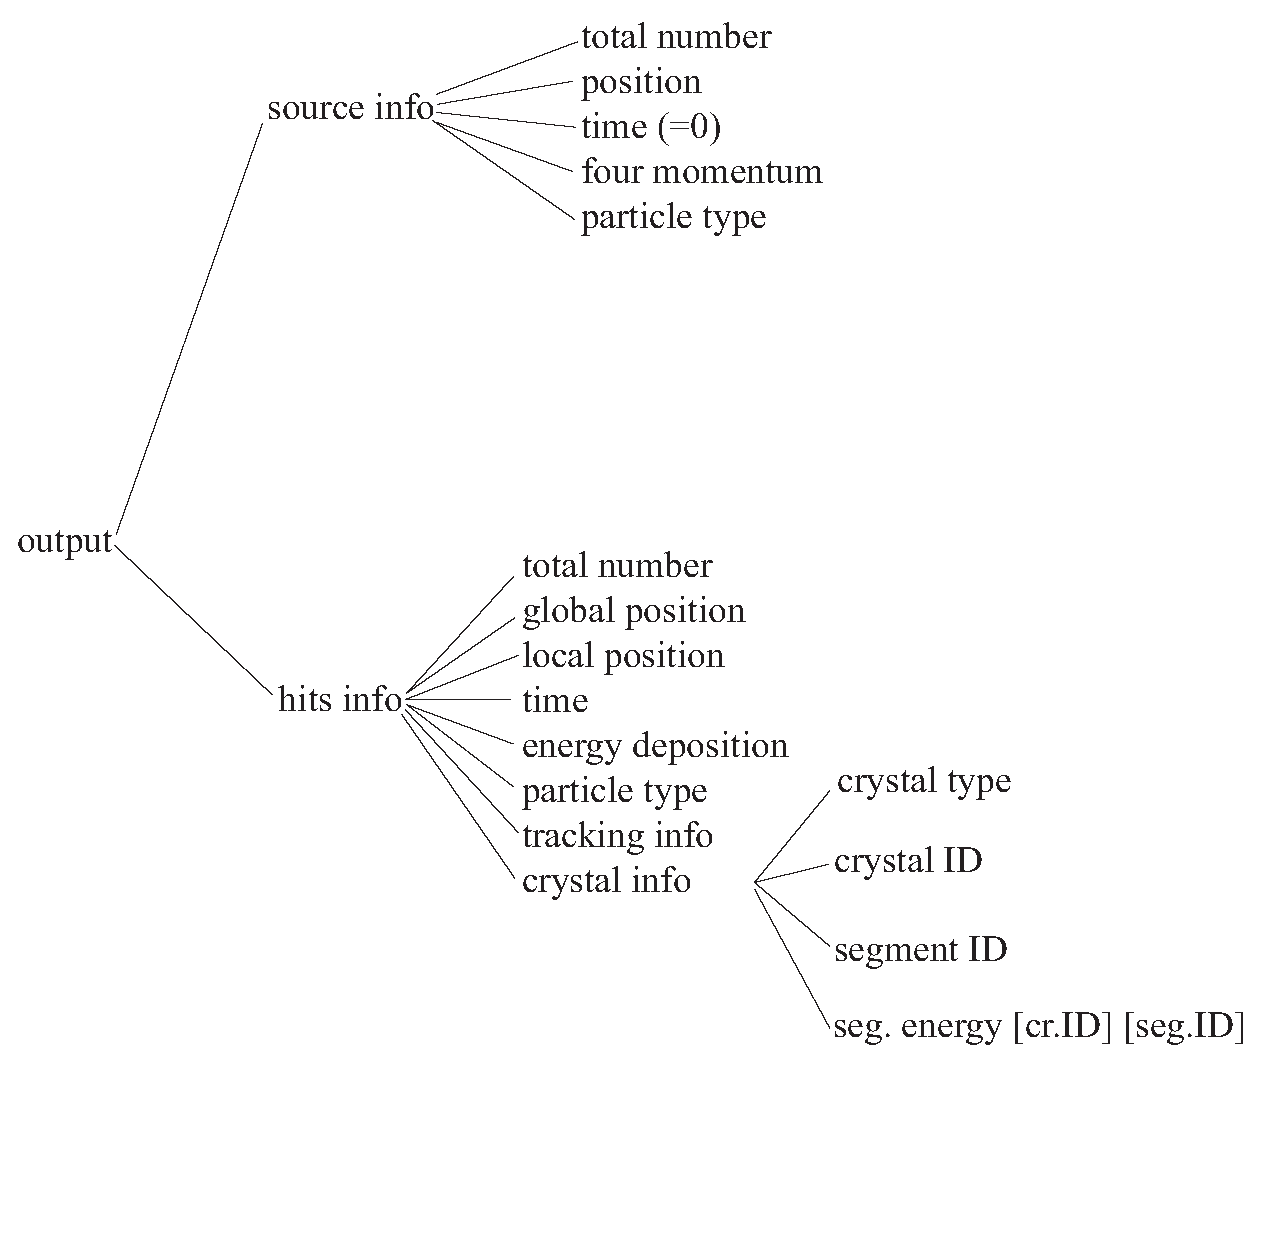
\includegraphics[scale=0.7]{figures/outputtree_big}
\caption{\small ROOT output tree of the class GEOutputCrystal. The segment energy is saved with respect to the crystal ID and the segment ID.}
\end{center}
\end{figure}

You can use the features of the class by typing:
\begin{lstlisting}
/MG/eventaction/rootscheme Crystal
/MG/eventaction/Crystal/save [source, hits, tracks, all]
\end{lstlisting}
\vspace{0.2cm}
The options in ``[  ]'' can be chosen from the ones listed above. You may use either one of them or a combination. In detail, they imply:\\
\begin{itemize}
 \item source - saves only the primary vertex and particles information
 \item hits - saves the hits and trajectories in the sensitive volumes
 \item tracks - saves all hits and all trajectories
 \item all - saves, well, all..
\end{itemize}
The default option is ``hits'', if the parameter is omitted.\\
\vspace{0.2cm}\\
Users can get the crystal type from the following ROOT branch:
\begin{lstlisting}
hitCrystalType[maxNhits]
\end{lstlisting}
The values correspond to the hit being in:
\begin{itemize}
\item -1 : not a sensitive volume at all
\item  0 : a sensitive volume but not a crystal
\item  1 : RolandI (unsegmented true coaxial p-type detector)
\item  2 : RolandII (6-fold segmented true coaxial p-type detector) 
\item  3 : RolandIII (18-fold segmented true coaxial p-type detector)  
\item  4 : Siegfried (18-fold segmented true coaxial n-type detector)
\end{itemize}
\vspace{0.2cm}
All the segments are arranged according to their local coordinate system. They are numbered from 1 for the first segment, R==0 and $\Phi$==0, counterclockwise and bottom up. The segmentation scheme and the segment numbering of the crystal ``Siegfried'' are shown in figure \ref{fig:segscheme}. Every event in a crystal is assigned to a detector segment according to the segmentation scheme using its z-, R- and $\Phi$- values.\\
\begin{figure}[h!]
 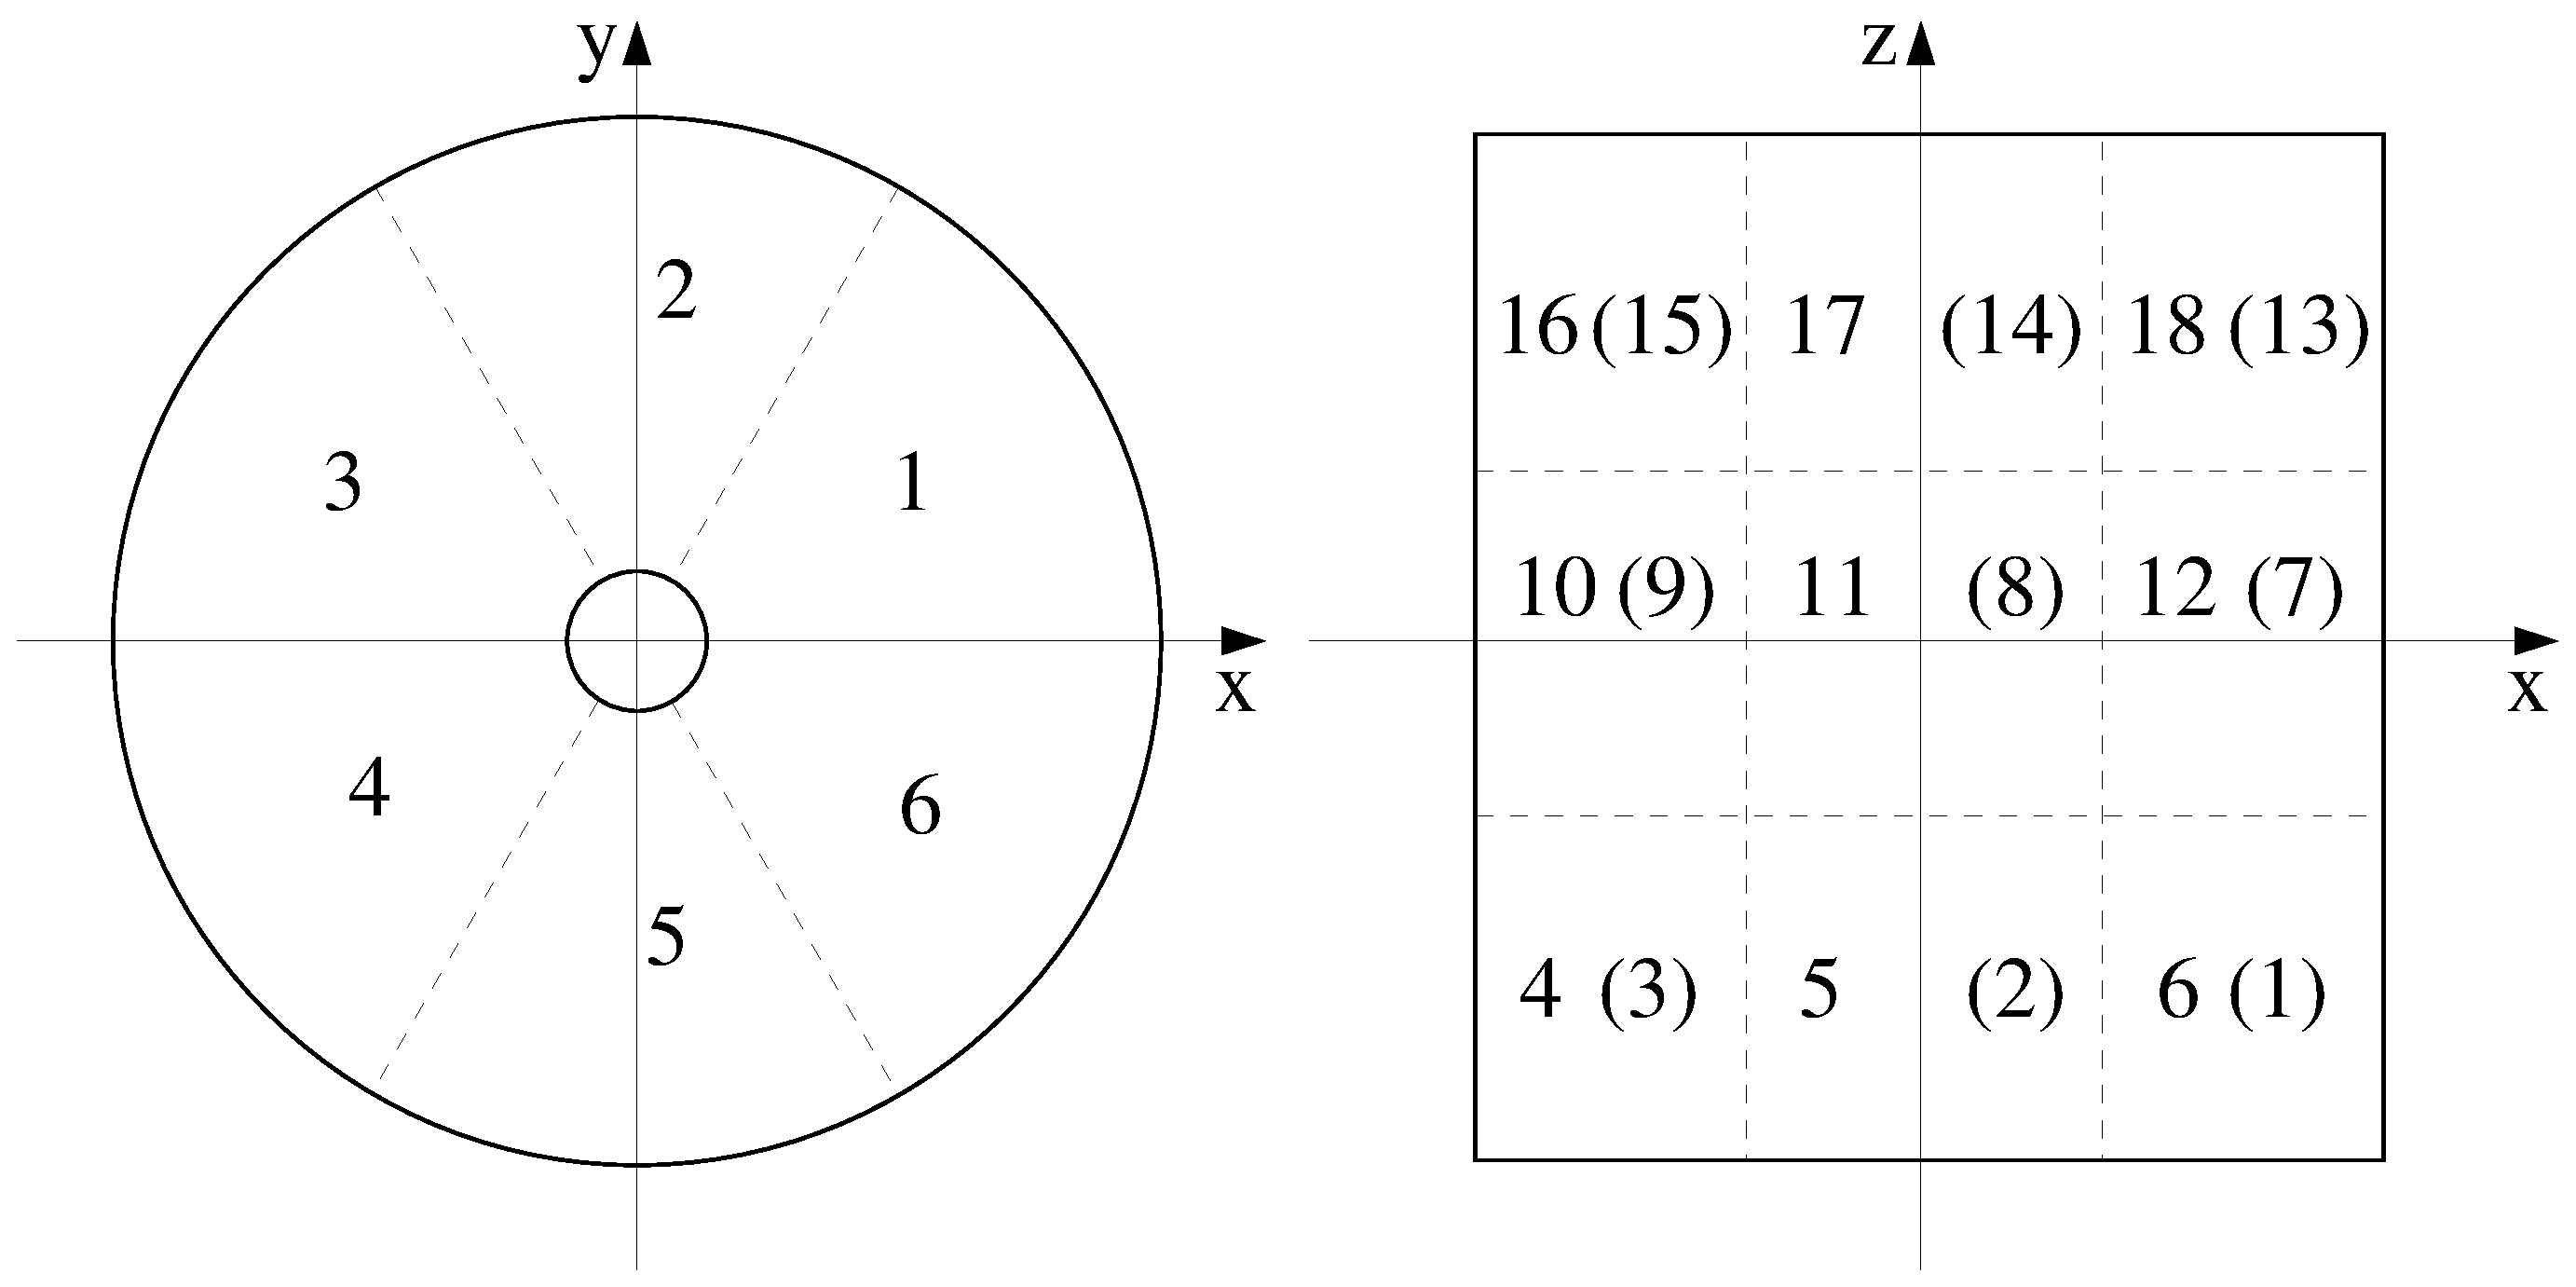
\includegraphics[scale=.3]{figures/segSchema}
\caption{Segmentation scheme for ``Siegfried''}
\end{figure} \label{fig:segscheme}
The segment shown in the ROOT branch is specified by the parameter:
\begin{lstlisting}
hitSegmentID[maxNhits]
\end{lstlisting}
The values correspond to:
\begin{itemize}
\item  -1 : not a sensitive volume at all
\item 0 : the whole volume which is sensitive (the whole detector)
\item 1 : the first segment  
\item 2 : the second segment
\item  ...
\end{itemize}
\vspace{0.2cm}
The crystal position in the \gerda \ array is given in the ROOT branch:
\begin{lstlisting}
hitCrystalID[maxNhits]
\end{lstlisting}
The values correspond to:
\begin{itemize}
\item -1 : not a sensitive volume at all
\item 0 : sensitive volume but not a crystal
\item 1 : the first crystal
\item 2 : the second crystal
\item  ...
\end{itemize}
The energy deposited in a segment of a crystal is saved in the ROOT branch:
\begin{lstlisting}
segmentEnergy[crystalID][segmentID]
\end{lstlisting}
Only positive crystal IDs can be used here, of course (negative values are not sensitive volumes). For crystal ID = 0, only segment ID = 0 is available (a volume with crystal ID = 0 is not a crystal). Crystal ID = n and segment ID = 0 shows you the energy deposited in the complete  n$^{th}$ crystal.\\
\subsubsection{Geometry developers' guide}
The implementation of segmentation and sensitive volumes is the pat that interests a developer. How this is done is explained here in a few steps.\\
The definition of a logical volume and a physical volume in \mage \ works as follows:\\
The geometry of a crystal is defined. It becomes a logical volume with attributes in the geometry construction class, e.g. in ``GEMunichTestStandDB'':
\begin{lstlisting}
fCrystalLogical 
= new G4LogicalVolume(CrystalTubs,	   //the name of the created geometry
		      enrichedGermanium,   //the material the crystal consists of
		     "CrystalLogical");	   //its name
\end{lstlisting}
This logical volume is inserted in the physical volume that is constructed like this:
\begin{lstlisting}
fCrystalPhysical
  = new G4PVPlacement(0, 			     //no rotation
		      G4ThreeVector(0,0,0),	     //translation position
		      fCrystalLogical,		     // pointer to its logical vol.
		      "CrystalPhysical",	     //its name
		      fCrystalMotherVolumeLogical,   //its mother logical volume
		      false,			     //no boolean operations
		      0);			     //its Copy Number
\end{lstlisting}
The physical volume name of a crystal defines its type. The class recognizes this and creates a segmentation scheme according to the
type. You don't have to define each segmentation in your geometry construction class.\\
You can take a simple G4Tubs object and name the physical volume ``siegfried''. The segmentation scheme predefined as ``siegfried''- scheme is implemented on the crystal. This means that hits inside this crystal have a segment ID according to their positions and the ``siegfried'' segmentation scheme.\\
A sensitive volume will be automatically recognized by the class from a physical volume.
You can change a usual physical volume to a sensitive one very easily: You only have to rename it as: ``PhysicalVolume'' $\longrightarrow$ ``sensitive\_PhysicalVolume''.\\
The hits in a sensitive volume are assigned to the segment of a detector using their local coordinates with the origin at the geometric center of the crystal:  x$_i$, y$_i$, z$_i$, T$_i$, p$_{x,i}$, p$_{y,i}$, p$_{z,i}$ and E$_{k,i}$ for the i$^{th}$ hit. The local coordinate system is also given in R$_i$, $\Phi$ $_i$ and z$_i$ with z$_i$==0 at half the height of the crystal.\\
The \gerda \ array consists of more than one detector. The position of each crystal is defined by its "CopyNo.".\\
Detectors in LAr are characterized by their logical volumes inside the mother volume "LAr" that are numbered top to bottom: 0, 1, 2... Hits inside these volumes will have a crystal ID (equals the CopyNo.+1): 1, 2, 3...\\
\vspace{0.2cm}\\
The definition of a physical volume in reality might look like this:
\begin{lstlisting}
fCrystalPhysical
  = new G4PVPlacement(0, 			     
		      G4ThreeVector(0,0,0),	     
		      fCrystalLogical,		     
		      "sensitive_siegfried",	     
		      fCrystalMotherVolumeLogical,   
		      false,			     
		      1);			     
\end{lstlisting}
The class GEOutputCrystal extracts the following information from this physical volume:\\
\begin{itemize}
\item It is a sensitive volume with the segmentation scheme of the crystal siegfried (the \textbf{crystal type }is defined).
\item The copy number of the crystal is 1, its \textbf{crystal ID} is 2 according to the scheme mentioned above.
\end{itemize}
If a hit is in segment 15 of ``Siegfried'', for example, this means:
\begin{itemize}
\item hitCrystalType = 4
\item hitCrystalID = 2
\item hitSegmentID = 15
\end{itemize}



\section{Majorana Output}
\label{IO_Majorana}


% -------------------------------------------------------- 
% materials  
% --------------------------------------------------------  

\chapter{Material definitions}
\label{chapter:materials}
{\it tba} \\ 
\input{materials.tex}


% -------------------------------------------------------- 
% detector components  
% --------------------------------------------------------  

\chapter{Detector components}
\label{chapter:detector}
{\it all} \\ 
\section{MGGeometry Classes}

 The following is a list of classes in the MGGeometry framework and
a description of their uses.


MGGeometryDetectorConstruction
 
\begin{lstlisting}
    This class is the primary class that builds the MG materials as
    well as instantiates any detector chosen in the
    /MG/geometry/detector messenger described above. It creates a
    world volume and places the detector as a single object inside
    it. Eventually it will first place a shield inside the world
    volume, and then a detector inside the shield, but for now we
    don't have any shields.
   \end{lstlisting}

MGGeometryDetector

\begin{lstlisting}
    This is the base class for all MGGeometry detector classes.
    When instantiated, it must be called with the serial number of
    the desired detector. It allocates a pointer to the outermost
    detector and sets its name. All other functionality must be built
                                within each individual kind of detector class.
   \end{lstlisting}
MGGeometryDetectorMessenger
 
\begin{lstlisting}
    The object that is used to issue commands to the MGGeometry
    framework.
   \end{lstlisting}
MJGeometry800gCrystal MJGeometryCloverDetector MJGeometryCloverInNaIBarrel MJGeometrySolidBlock
 
\begin{lstlisting}
    These are subclasses of the MGGeometryDetector class. These
    classes may contain active detector subparts (e.g.,
    the MJGeometryCloverDetector), but as far as the simulation is
    concerned, these classes correspond to the ``entire'' detector
    detector. (``Entire'' is in quotes because what makes up the
    ``entire'' detector is somewhat subjective. A dewar, for instance,
    may or may not be thought of as part of the detector.)
   \end{lstlisting}
    MJGeometryCloverCrystal
   MJGeometryNaIBarrel
 
\begin{lstlisting}
    These classes are subparts of detectors. For examples, the
    MJGeometryCloverDetector contains pointers to four
    MJGeometryCloverCrystals, and each crystal is treated as a
    separate object. When the four crystals are instantiated as
    part of the MJGeometryCloverDetector, however, the entire
    clover detector is handled as as object incorporating the
    crystals.
   \end{lstlisting}
  

\section{GERDA Geometry}

The GERDA geometry can be chosen by setting the command
 
\begin{lstlisting}
   /MG/geometry/detector [detector]
                    \end{lstlisting}
 in the corresponding macro. For the
standard GERDA geometry, the detector has to be ``GerdaArray". Also
other geometries exist that are related to the GERDA experiment,
i.e. they are either modified geometries or teststands.


The geometry is organized in a group of classes: the following figure gives an
overview of the structure.  
\begin{figure}
\begin{center}
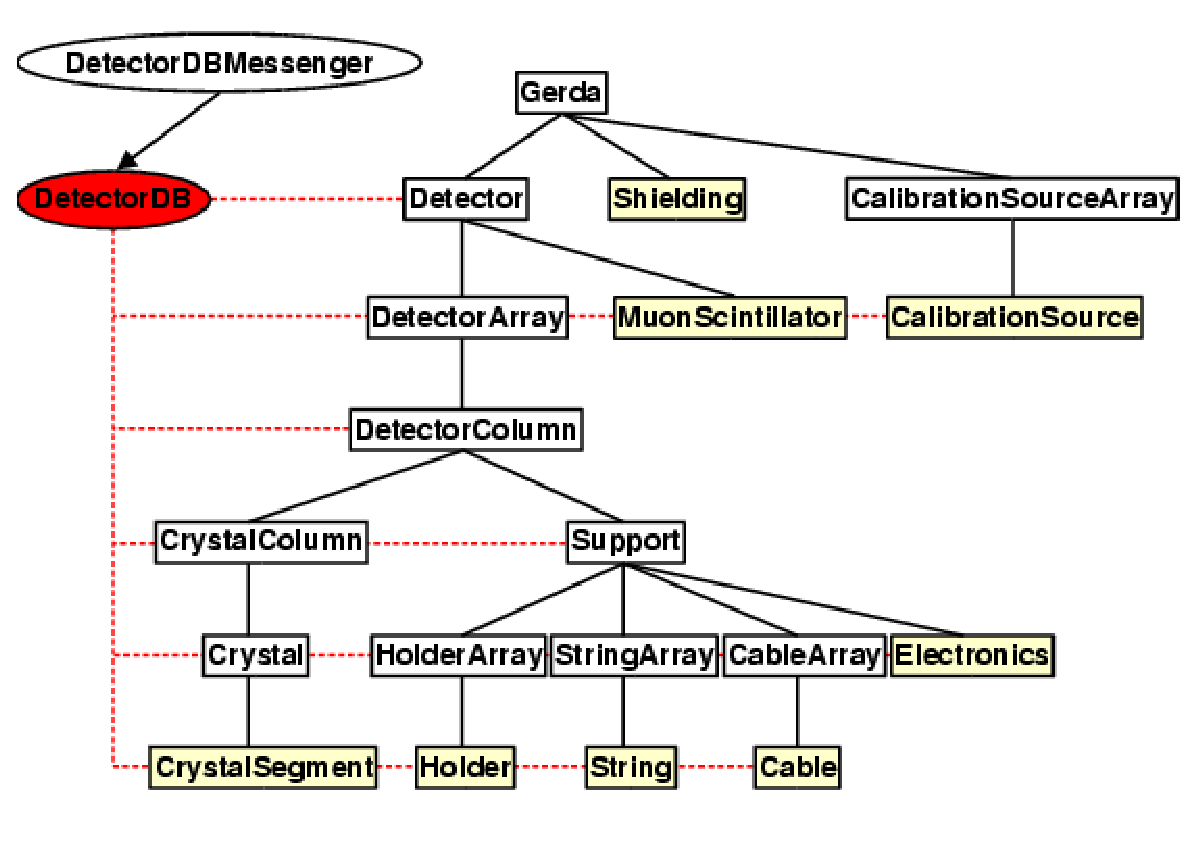
\includegraphics[width=.8\textwidth]{geometryclasses}
\end{center}
\caption{Class structure for GerdaArray}
\end{figure}
The class names in the figure do not
include the prefix GEGeometry since it is common to all classes
displayed. The class ``GEGeometryGerda" inherits from
``MGGeometryDetector", i.e. it is the basic class which gets
instantiated from the MaGe framework. Since the real geometry of the
experiment is still under investigation and not fixed yet, the Monte
Carlo is kept as flexible as possible. For that reason a database
class, ``GEGeometryDetectorDB" is introduced which governs all the
parameters for the geometry. Those parameters can be adjusted by
commands, i.e. there exists a messenger class which controls the
database. As can be seen in the diagram, the database is connected to
all classes in the geometry structure.


The first three branches ``Detector", ``Shielding" and
"CalibrationSourceArray" are rough groupings. In order to focus on
particular parts of the geometry each of those branches can be 
switched off. The calibration sources for example are not needed for 
the study of internal background of the crystals and the support.
The detector itself consists of an array of crystals which is made out
of bare crystals (or crystal segments) and a support structure that
includes holders, strings, cables and electronics. This allows easy
replacements of parts of the geometry for test reasons or changes in
the setup.  Auxiliary detectors are also installed, namely the muon
plastic scintillator on top of the vessel and photomultipliers inside
the water tank (not yet in the Monte Carlo).
The shaded classes are those in which physical volumes are
created. Also, most of the calculations for positioning and
orientation are done via class functions.
In order to add new elements to the simulation new classes are added.
Existing examples are the scintillator and the germanium
detectors. The solids and logical volumes should be introduced in the
database class whereas the physical volume should be instanciated in
the corresponding class. All used parameters are held flexible by
adding the corresponding commands to the database messenger
class. This has to include a flag that controls if the new element is
to be included in the run or not. By following these instructions, the
changes can be submitted to the CVS repository and are made available
for other users


 The following setups are currently available. They are defined by the
settings in the corresponding macros, i.e. the deviation from the
default values of the geometry parameters.
 Phase I:           Unsegmented crystals. So far, this setup is only used in the study of cosmic muons.
 Phase II:          7 strings with 3 crystals. Each crystal is segmented into 6 phi-{} and 3 z-{}segments (standard).
 Simple Test Stand: A standard crystal within an aluminum cryostat which is placed in front of a capsulated
       source and lead bricks. The comparison of Monte Carlo and real data provided a first
       validation of the new MaGe code development.
 
\section{Germanium detectors} 
{\it Kevin} \\ 

\section{Muon veto}
\begin{table}[ht]
 \caption{Overview over the different photomultiplier distributions for the Cherenkov veto for GERDA. \label{Table:pmt_dist}}
 \begin{center}
  \begin{tabular}{|c|c|c|l|}
   \hline
   distributionnumber  & \# of pmts in pillbox & \# of pmts in water & comment \\ \hline \hline
   0                   &                     6 &                  66 & standard distribution \\ \hline
   1                   &                     4 & 70                  & alternative distribution \\ \hline
   -1                  &                     0 &                   0 & no Cherenkov veto \\ \hline
  \end{tabular}
 \end{center}
\end{table}
The GERDA muon veto consists out of two systems. The plastic scintillator panels on top of the penthouse 
and the Cherenkov veto in the water tank surrounding the cryostat. In \mage the plastic panels are hard
coded in the geometry structure, while the Cherenkov veto has some commands to activate it or to select a
different placement of the photomultipliers in the water tank. \\
The photomultipliers in the GERDA geometry are currently constructed out of stainless steel housings and a PET-foil 
covering the upper part of the PMTs. If a photon hits the PET foil, a hit is scored and written into the output file. 
To account for the efficiency of the photomultiplier, it is recommendened to kill four of five photons in the MGManagmentStackingAction.cc, to save simulation time. Otherwise the efficiency has to be considered in the analysis 
of the root files. \\
Currently there are two different distributions, the user can select (see table \ref{Table:pmt_dist}), or one
can simply deactivate the Cherenkvo veto. 

The Cherenkov veto is initiated with the macro command:
\begin{lstlisting}
/MG/geometry/cherenkov distributionnumber
\end{lstlisting}
Of course, the optical processes have to be activated with
\begin{lstlisting}
/MG/processes/optical true
\end{lstlisting}
and the optical output has to be selected:
\begin{lstlisting}
/MG/eventaction/rootschema GerdaArrayOptical
\end{lstlisting}
Otherwise no Cherenkov effect takes part, and no photons are registered with the photomultipliers.
The data is than accumulated in the root output file in the branches \textit{ph\_$\star$} and 
\textit{PMT\_$\star$} for the Cherenkov veto and in the branch \textit{$\star$\_\ scint \_$\star$} for
the plastic panels.


\section{Electronics and calibration sources} 
{\it Daniel} \\ 

\section{Infrastructure} 
{\it Jens} \\ 



% -------------------------------------------------------- 
% test stands 
% --------------------------------------------------------  

\chapter{Test stands}
\label{chapter:teststands}
{\it all} 

\section{Existing test stands}

\section{How to add a test stand to MaGe}

% -------------------------------------------------------- 
% bibliography
% -------------------------------------------------------- 

\clearpage
\addcontentsline{toc}{chapter}{Bibliography}

\begin{thebibliography}{99}
%
\bibitem{Agostinelli:2002hh}
  S.~Agostinelli {\it et al.}  [GEANT4 Collaboration],
  ``GEANT4: A simulation toolkit,''
  Nucl.\ Instrum.\ Meth.\ A {\bf 506} (2003) 250.
%
\bibitem{Allison:2006ve}
  J.~Allison {\it et al.},
  ``Geant4 developments and applications,''
  IEEE Trans.\ Nucl.\ Sci.\  {\bf 53} (2006) 270.
%
\bibitem{geant4physics}
  Physics Reference Manual,
  available at http://geant4.web.cern.ch/geant4.
%
\bibitem{Amako:2005xf}
  K.~Amako {\it et al.},
  ``Comparison Of Geant4 Electromagnetic Physics Models Against The Nist
  Reference Data,''
  IEEE Trans.\ Nucl.\ Sci.\  {\bf 52} (2005) 910.
% 
\bibitem{Amako:2006nb}
  K.~Amako {\it et al.}  [GEANT4 Collaboration],
  ``Geant4 and its validation,''
  Nucl.\ Phys.\ Proc.\ Suppl.\  {\bf 150} (2006) 44.
%
\bibitem{Lipari:1997}
  P.~Lipari and T.~Stanev, 
 Phys. \ Rev. \ D \textbf{44} (1991) 3543.
%
\bibitem{Kudryavtsev:1997}
 Astropart. Phys. \textbf{7} (1997) 357. 
%
\bibitem{Wulandari:2004}
 H.~Wulandari \emph{et al.}, 
 hep-ex/0401032 v1

\end{thebibliography}




%--------------------------------------------------------

\end{document}

%-------------------------------------------------------- 
 


